\section{Reglervalidierung} \label{sec:reglervalidierung}

Ziel der Reglervalidierung ist das Bestätigen des Regelverhaltens der modellierten drei Regler aus dem \autoref{sec:Zustandsreglerentwurf}. Dies wird mit Hilfe des Matlab Tools \textit{Simulink} durchgeführt. Die zuvor in Matlab Berechneten Matrizen (siehe \zB \autoref{eq:Gleichung41}) werden an das Simulink-Modell übergeben und dort genutzt. Die Simulationsergebnisse werden anschließend auf ihre Plausibilität geprüft. Dazu werden zum einen die Eingangsparameter (Anfangsauslenkung und Referenzposition) variiert und zum anderen wird der jeweilige Regler am linearen als auch am nichtlinearen Modell getestet.

\subsection{Validierung des linearen Modells}

Zunächst findet die Validierung der Regler am linearen Zustandsraummodell der Strecke statt. Die Simulink Implementierung der linearen Regelstrecke ist in \autoref{fig:Bild3} dargestellt.

\subsubsection{Zustandsregler mit einfacher Rückführung} \label{sec:val-acker}

Der erste Regler ist erneut der einfache Zustandsregler mit Rückführung. Dessen Implementierung in Simulink kann in \autoref{fig:Bild13} nachvollzogen werden. Als Simulationsergebnisse werden zum einen der Winkel des Pendels $\varphi$, die Wagenposition $x_{\mathrm{M}}$ und die benötigte Eingangskraft $u$ \bzw $F_{\mathrm{a}}$ in Diagrammform dargestellt. \\
Um das Verhalten des Reglers zu testen, wird die Simulation für verschiedene Anfangsauslenkungen des Pendels simuliert. Es wird untersucht, für welche Polstellen des Reglers welche Anfangsauslenkungen maximal eingeprägt werden dürfen, dass die Grenzen der Anlage nicht überschritten werden. Ziel ist es, zu bestätigen, welche Störung des Pendels (Abweichung des Winkels von der oberen Ruhelage) maximal auf dieses einwirken darf, so dass weder die maximale Eingangskraft von 80 N noch die maximale Wagenposition von $\pm$1 m überschritten wird. Dabei gilt es, die Polstellen nicht zu weit nach links auf der Real-Achse zu schieben, da dies den Regler beschleunigen würde. Dies führt jedoch zu größeren wirkenden Kräften und Momenten.

\begin{figure}[H]
    \centering
    \fbox{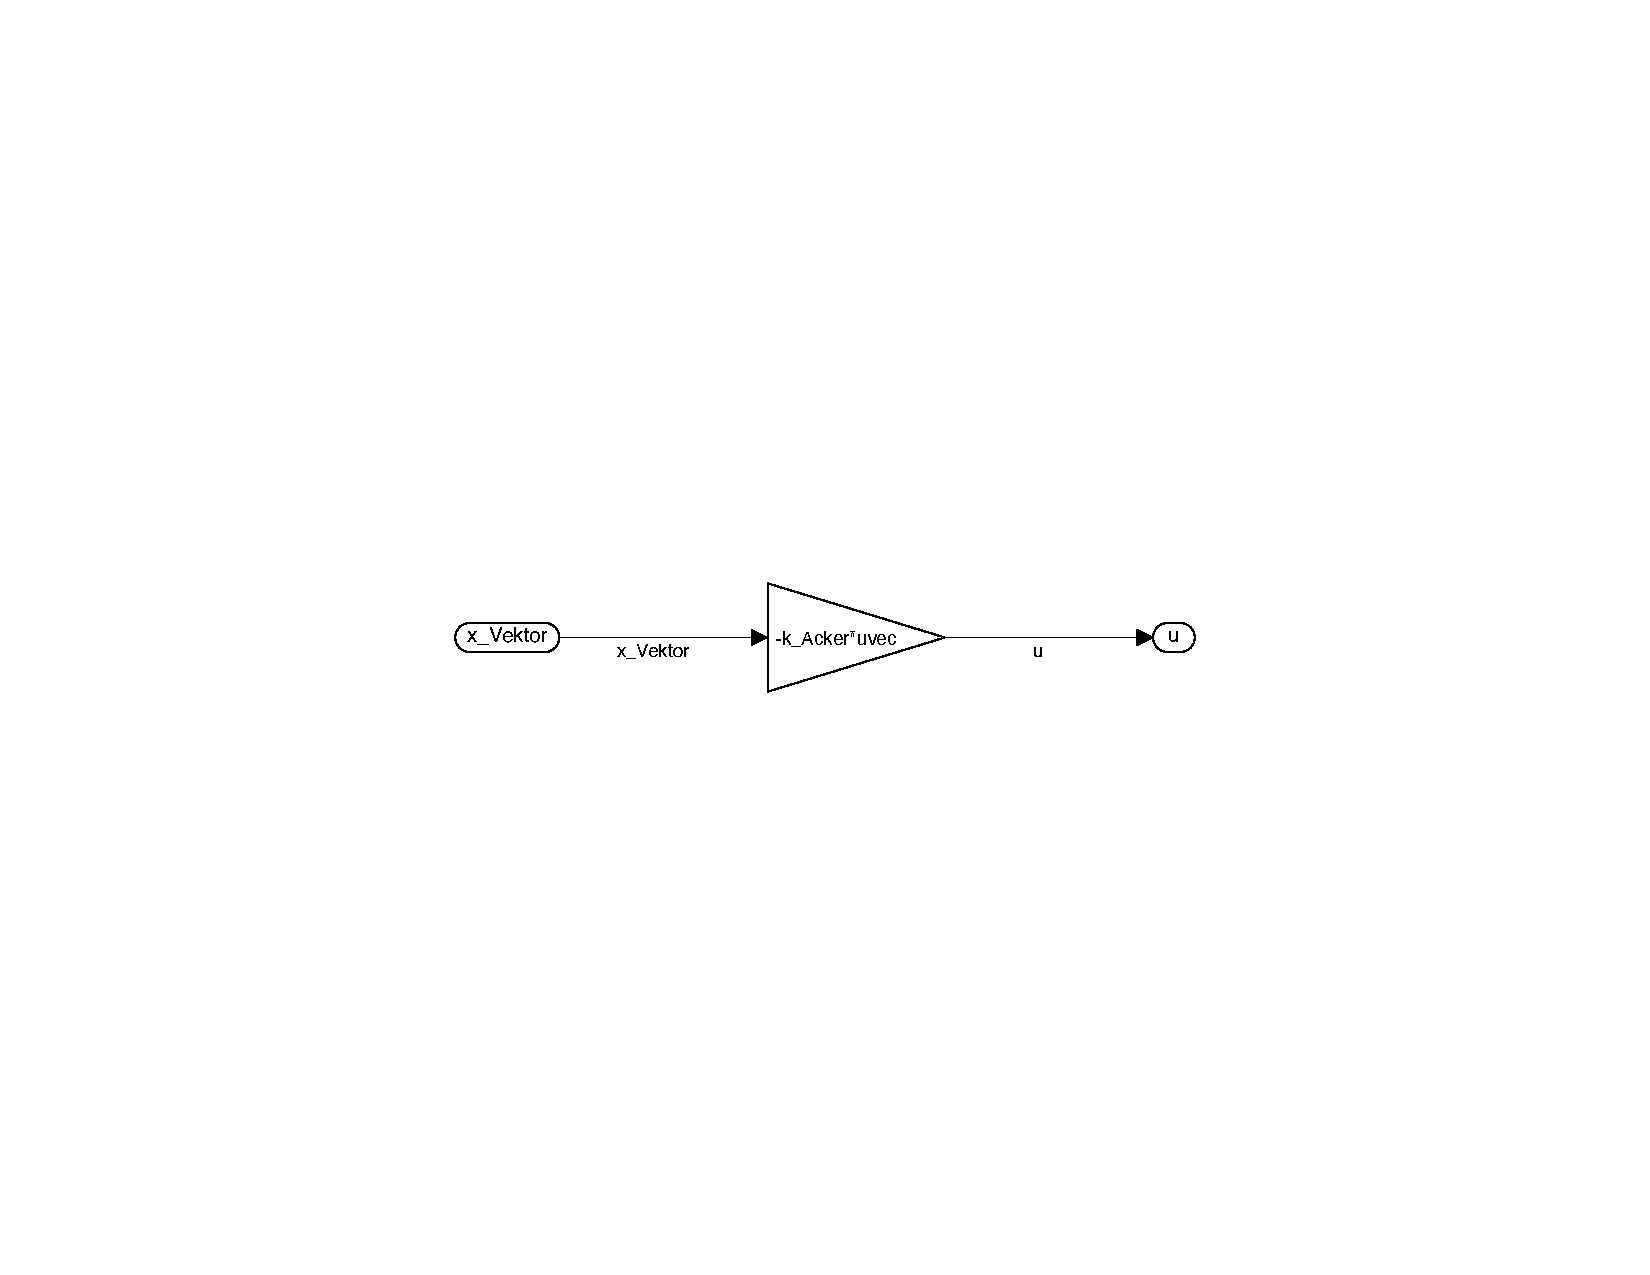
\includegraphics[width=0.7\textwidth]{Bilder/Reglervalidierung/Ackermann_Regler.pdf}}
    \caption[Einfacher Zustandsregler Simulink (linear)]{Simulink Regler-Blockschaltbild für den einfachen Zustandsregler (lineares Zustandsraummodell)}
    \label{fig:Bild13}
\end{figure}

\begin{figure}[H]
    \centering
    \fbox{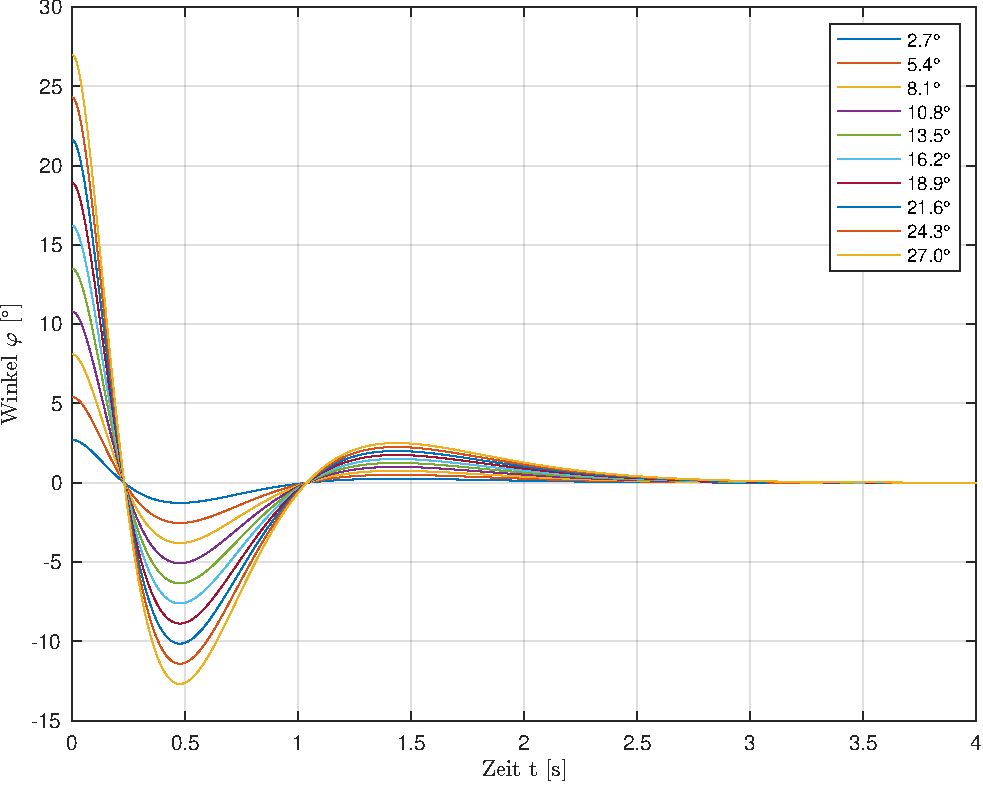
\includegraphics[width=0.6\textwidth]{Bilder/Reglervalidierung/linear_ackermann_phi.pdf}}
    \caption[$\varphi$ für einfachen Zustandsregler (linear)]{$\varphi$ für verschiedene Anfangsauslenkungen am einfachen Zustandsregler für das lineare Zustandsraummodell}
    \label{fig:Bild14}
\end{figure}

\begin{figure}[H]
    \centering
    \fbox{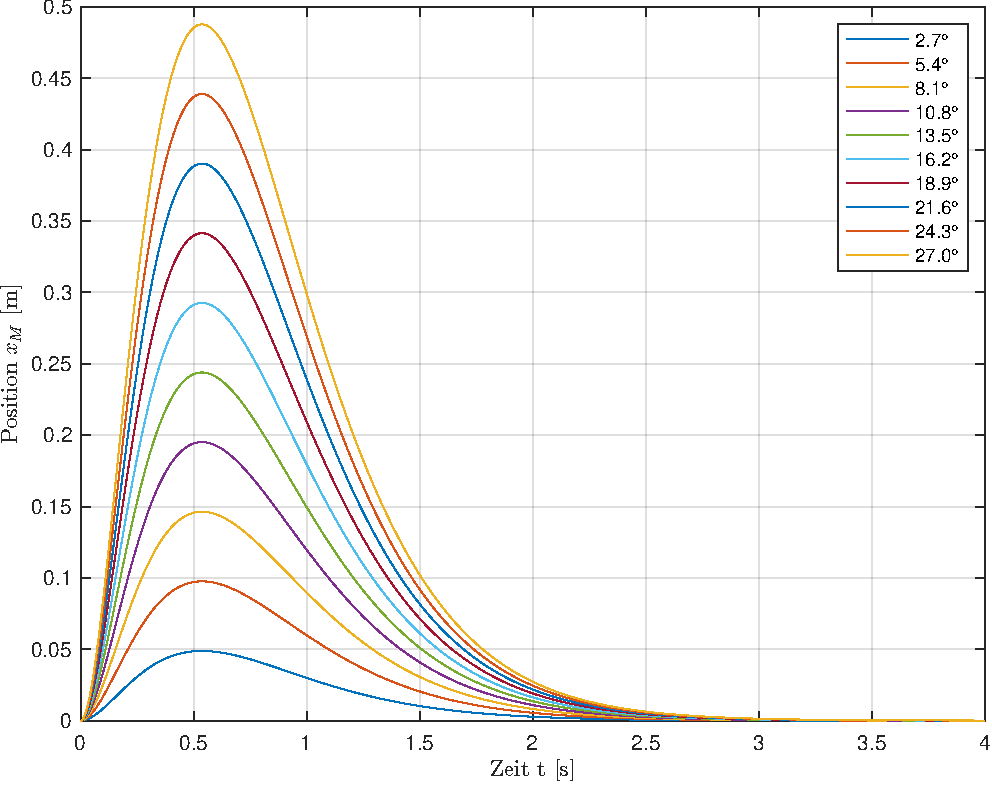
\includegraphics[width=0.6\textwidth]{Bilder/Reglervalidierung/linear_ackermann_xM.pdf}}
    \caption[$x_{\mathrm{M}}$ für einfachen Zustandsregler (linear)]{$x_{\mathrm{M}}$ für verschiedene Anfangsauslenkungen am einfachen Zustandsregler für das lineare Zustandsraummodell}
    \label{fig:Bild15}
\end{figure}

\begin{figure}[H]
    \centering
    \fbox{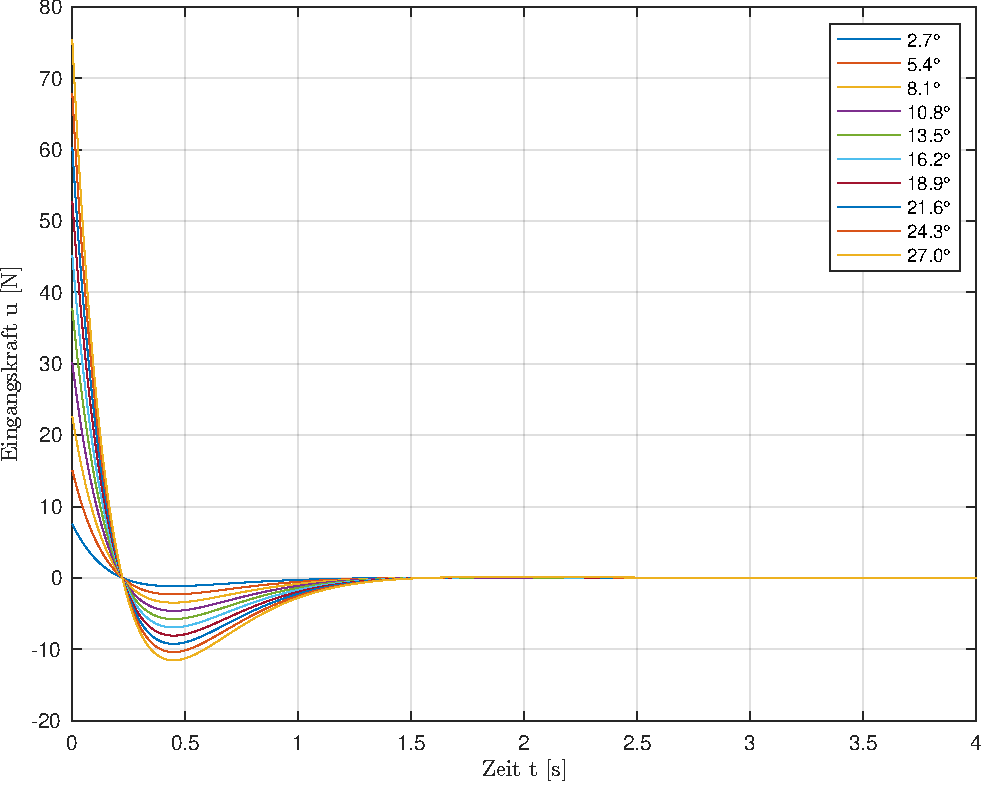
\includegraphics[width=0.6\textwidth]{Bilder/Reglervalidierung/linear_ackermann_u.pdf}}
    \caption[u für einfachen Zustandsregler (linear)]{u für verschiedene Anfangsauslenkungen am einfachen Zustandsregler für das lineare Zustandsraummodell}
    \label{fig:Bild16}
\end{figure}

Die für die oben gezeigten Diagramme gewählten Reglerpolstellen sind in \autoref{eq:Gleichung37} gezeigt. \\
\newline
\autoref{fig:Bild14} bestätigt, dass der Regler wie definiert eine Anfangsauslenkung zu $0^\circ$ (obere Ruhelage) ausregeln kann. Dabei ist zu erkennen, dass der Winkel $\varphi$ des Pendels erst leicht überschwingt, bevor er abschließend ausgeregelt wird. Der gesamte Vorgang dauert \ca 3 s. \\
\newline
Das Verhalten des Wagens ist in \autoref{fig:Bild15} gezeigt. Zu erkennen ist, dass bei einer positiven Anfangsauslenkung eine Bewegung des Wagens nach rechts stattfindet. Die Wagenposition $x_{\mathrm{M}}$ nimmt dementsprechend positive Werte an. Es handelt sich dabei um das zu erwartende Verhalten. Weiterhin bestätigt die Abbildung, dass selbst für einen Auslenkungswinkel von $27^\circ$ die maximale Wagenposition nicht überschritten wird. Von möglichen 100 cm werden lediglich knapp unter 50 cm benötigt. Da der einfache Zustandsregler keine Referenzpositionen für den Wagen entgegennehmen kann, ist die Position dieses am Ende wieder der Nullpunkt. \\
\newline
Das dritte Diagramm (\autoref{fig:Bild16}) zeigt die benötigte Kraft des Motors am Schlitten, um den Wagen in entsprechender Zeit an die zuvor gezeigte Position zu bewegen. Zu erkennen ist, dass für einen Winkel von $27^\circ$ der Motor maximal belastet wird. Es werden \ca 80 N benötigt. Für kleinere Auslenkungen ist weniger Kraft nötig, da auch die Position des Wagens weniger signifikant vom Ausgangspunkt abweicht. Es fällt auf, dass die Initialkraft am größten ist. Dies ist zu erklären über die Beschleunigung des Wagens. Beim Abbremsen kommt es auch hier zu einem Überschwingen, welches durch die negative Beschleunigung zu erwarten ist. Zuletzt ist festzuhalten, dass bereits nach rund 1,5 s der Motor keine Kraft mehr liefern muss. Somit ist die Eingangskraft bereits nach \ca der Hälfte der Ausregelzeit wieder bei u = 0 N  angelangt.\\
\newline
Zusammenfassend kann bestätigt werden, dass sich der Regler erwartungsgemäß verhält und die Grenzen der Anlage bezüglich maximaler Position und Kraft nicht überschritten werden.

\subsubsection{Zustandsregler mit Referenzwert-Vorsteuerung} \label{sec:val-vor}

Nachfolgend soll der Regler mit Vorsteuerung validiert werden. Dessen Simulink-Struktur ist in \autoref{fig:Bild17} aufgezeigt. Im Unterschied zu \autoref{sec:val-acker} kann bei diesem Regler eine Referenzposition für den Wagen vorgegeben werden. \\
In Diagrammform werden erneut der Winkel des Pendels $\varphi$, die Wagenposition $x_{\mathrm{M}}$ und die benötigte Eingangskraft $u$ \bzw $F_{\mathrm{a}}$ dargestellt. Zusätzlich wird die Validierung für verschiedene Referenzpositionen $y_{ref}$ vorgenommen. \\
Ziel ist auch hier das Bestätigen des Einhaltens der Grenzen der Anlage für die gewählten Polstellen bei untersuchten Anfangsauslenkungen und Referenzpositionen. 

\begin{figure}[H]
    \centering
    \fbox{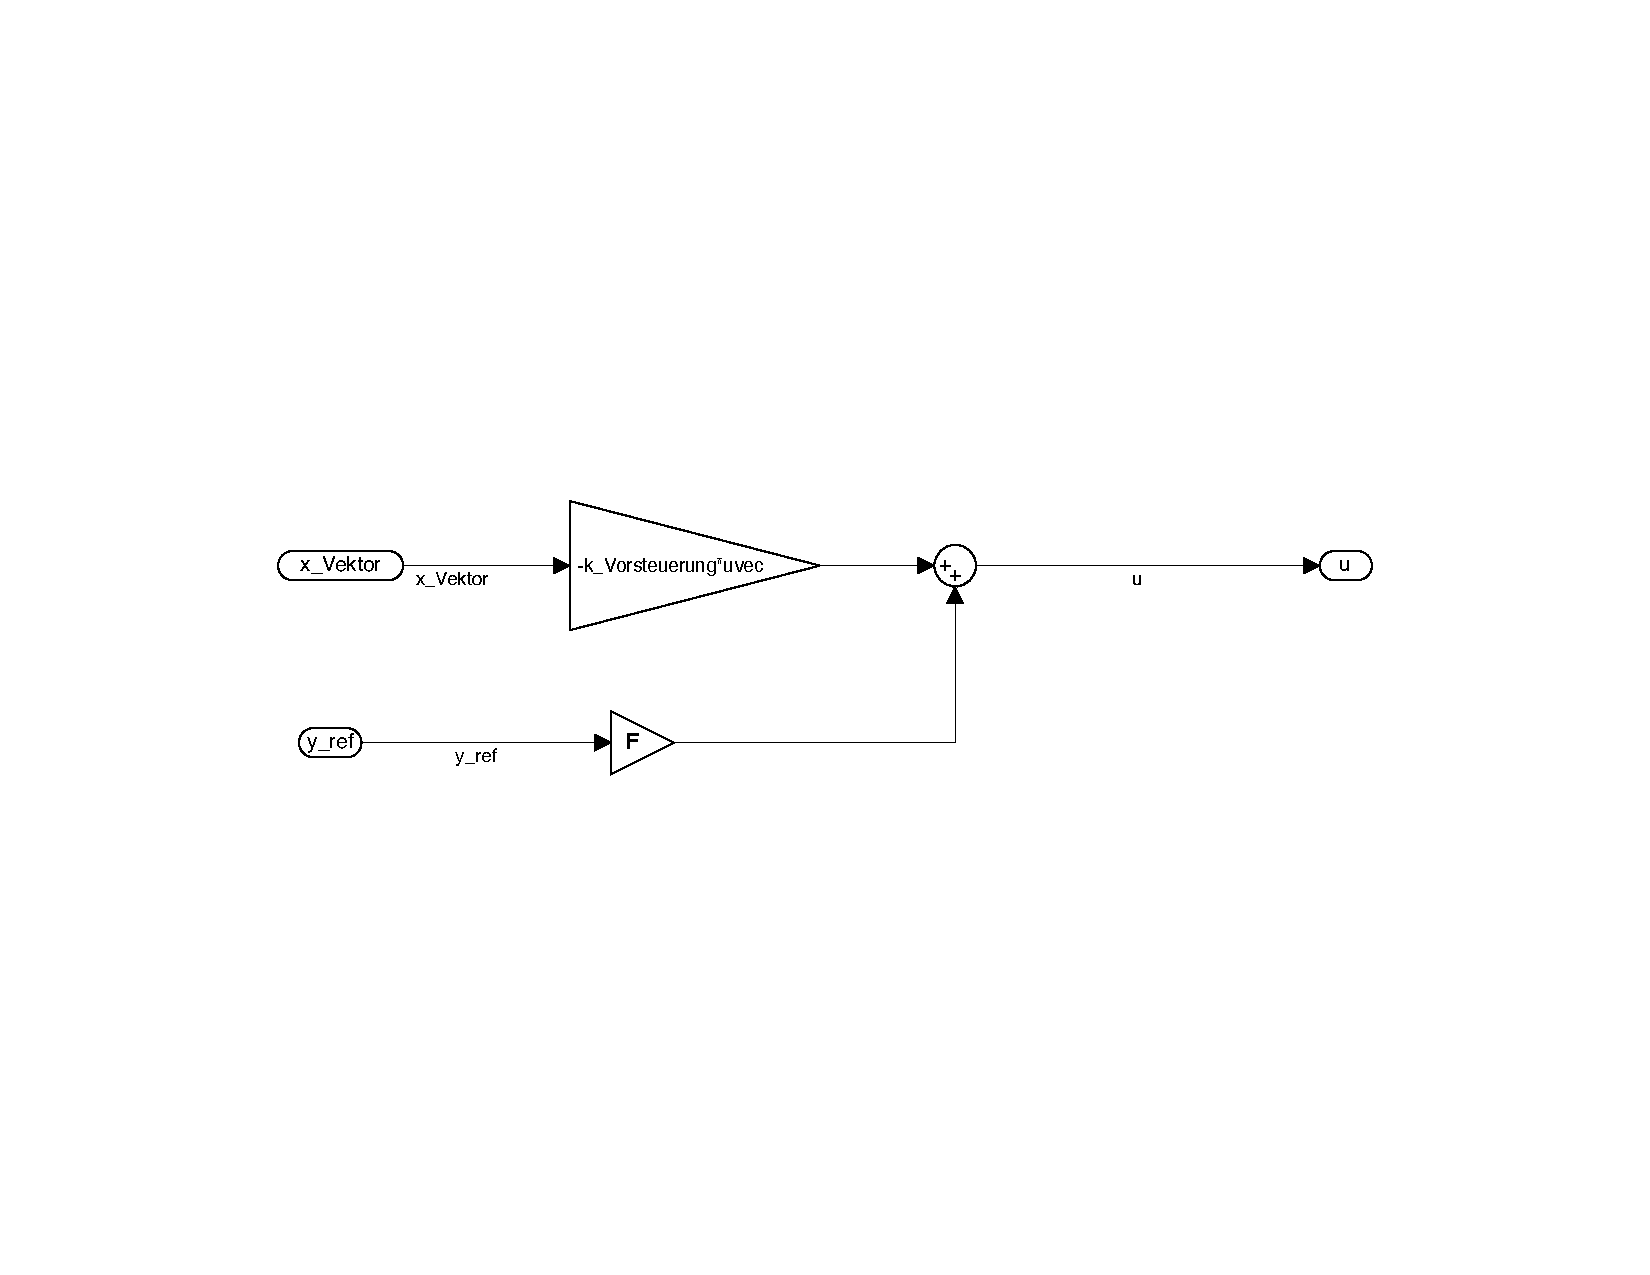
\includegraphics[width=1.0\textwidth]{Bilder/Reglervalidierung/Vorsteuerung_Regler.pdf}}
    \caption[Regler mit Vorsteuerung Simulink (linear)]{Simulink Regler-Blockschaltbild für den Zustandsregler mit Vorsteuerung (lineares Zustandsraummodell)}
    \label{fig:Bild17}
\end{figure}

\begin{figure}[H]
    \centering
    \fbox{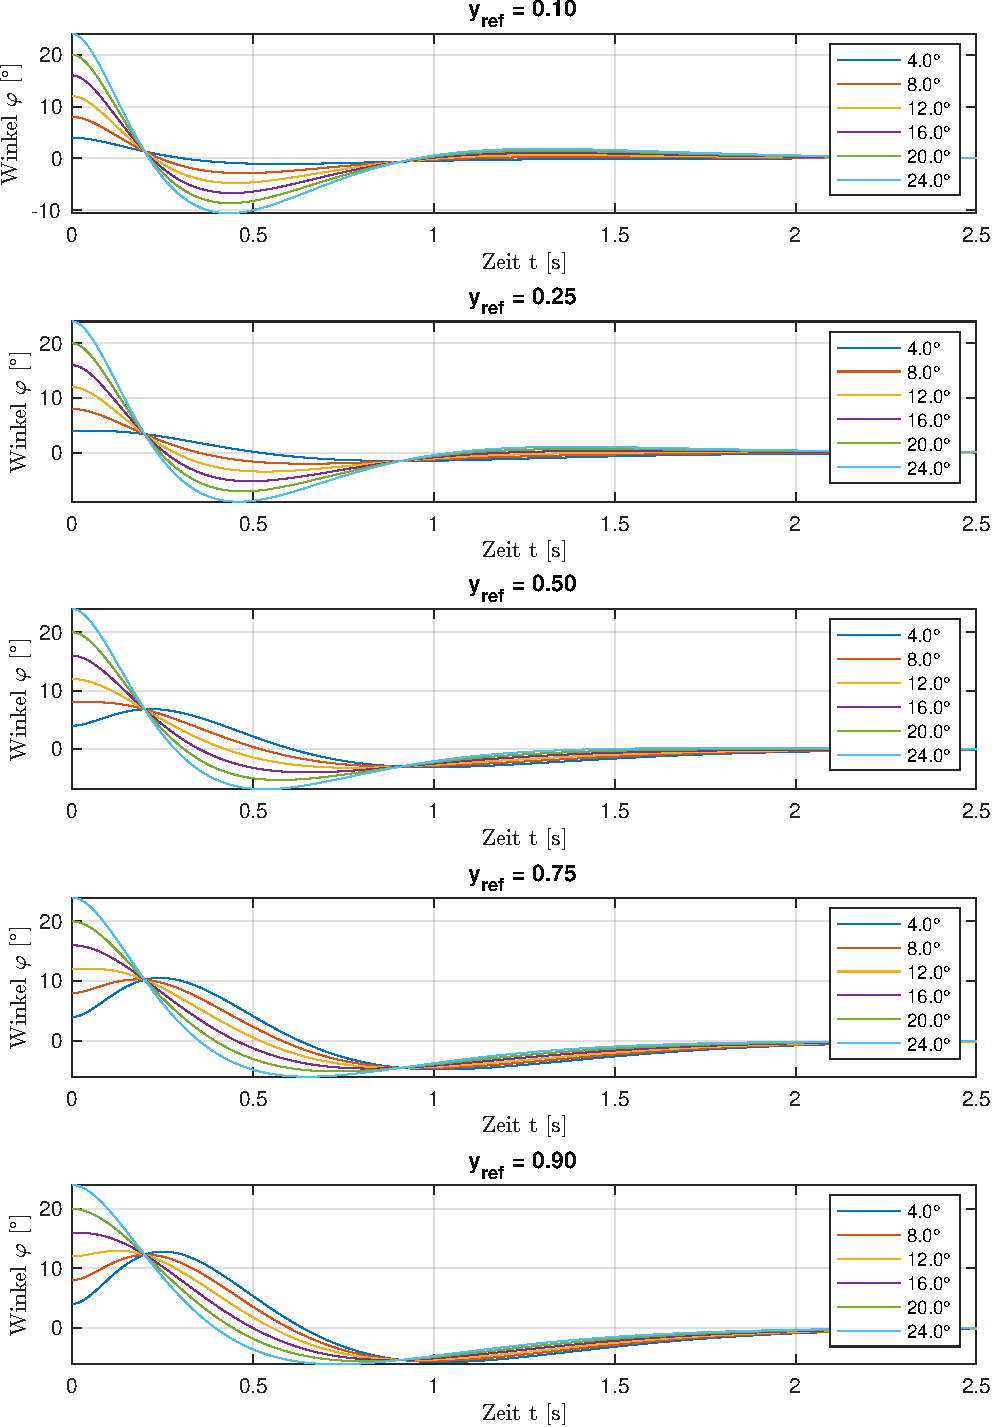
\includegraphics[width=0.76\textwidth]{Bilder/Reglervalidierung/linear_vorsteuerung_phi.pdf}}
    \caption[$\varphi$ für Regler mit Vorsteuerung (linear)]{$\varphi$ für verschiedene Referenzpositionen $y_{ref}$ und Anfangsauslenkungen am Zustandsregler mit Vorsteuerung für das lineare Zustandsraummodell}
    \label{fig:Bild18}
\end{figure}

\begin{figure}[H]
    \centering
    \fbox{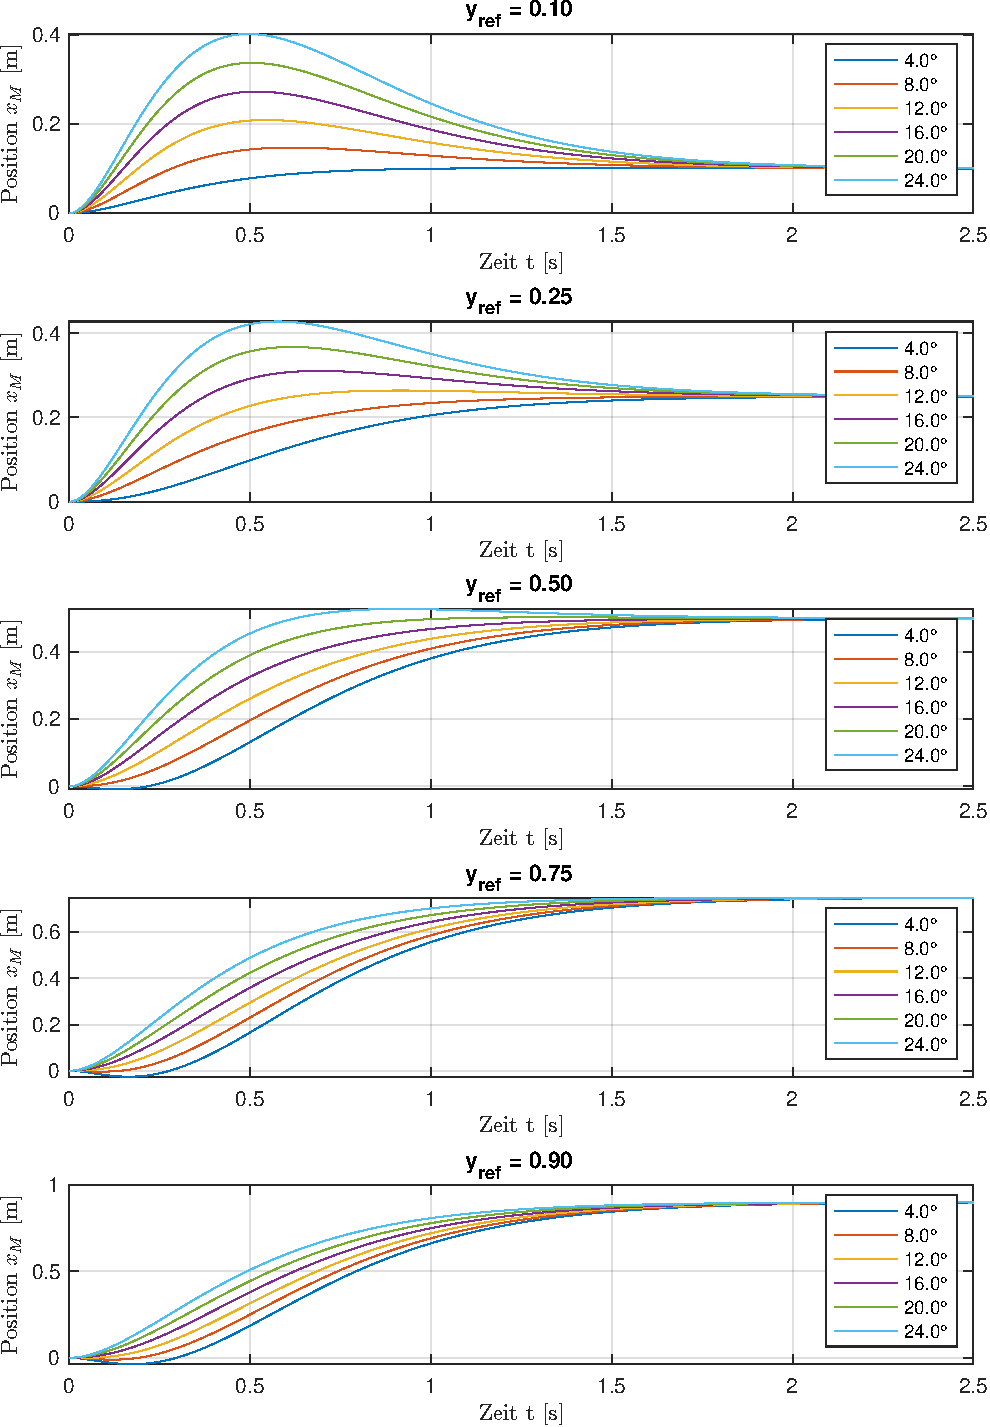
\includegraphics[width=0.76\textwidth]{Bilder/Reglervalidierung/linear_vorsteuerung_xM.pdf}}
    \caption[$x_{\mathrm{M}}$ für Regler mit Vorsteuerung (linear)]{$x_{\mathrm{M}}$ für verschiedene Referenzpositionen $y_{ref}$ und Anfangsauslenkungen am Zustandsregler mit Vorsteuerung für das lineare Zustandsraummodell}
    \label{fig:Bild19}
\end{figure}

\begin{figure}[H]
    \centering
    \fbox{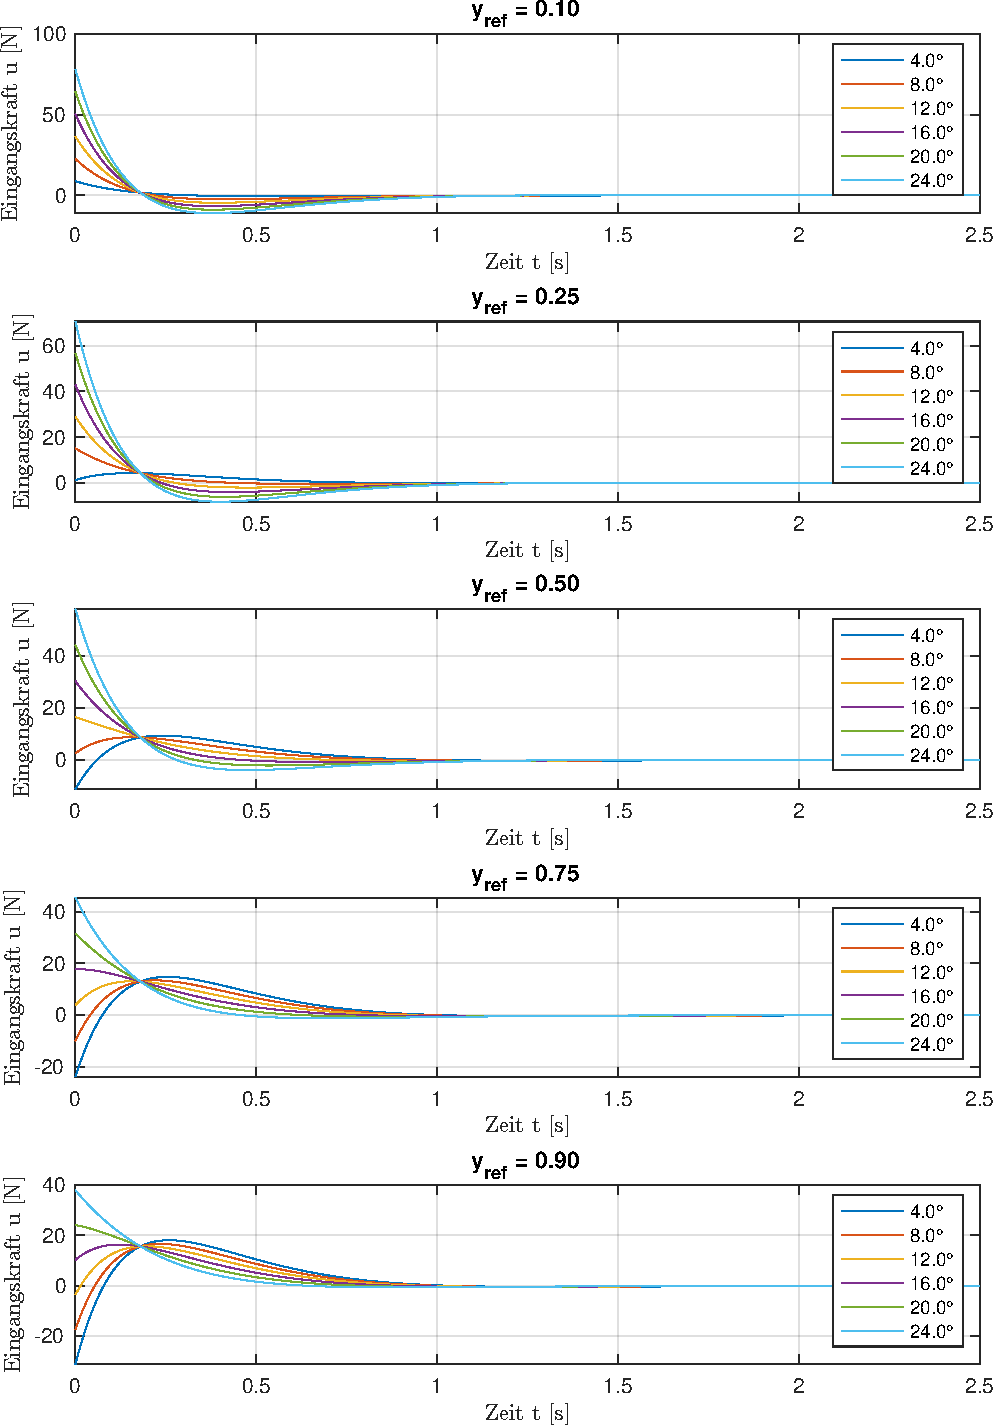
\includegraphics[width=0.76\textwidth]{Bilder/Reglervalidierung/linear_vorsteuerung_u.pdf}}
    \caption[u für Regler mit Vorsteuerung (linear)]{u für verschiedene Referenzpositionen $y_{ref}$ und Anfangsauslenkungen am Zustandsregler mit Vorsteuerung für das lineare Zustandsraummodell}
    \label{fig:Bild20}
\end{figure}

\newpage
Die für die oben gezeigten Diagramme gewählten Reglerpolstellen sind in \autoref{eq:Gleichung56} gezeigt. \\
\newline
\autoref{fig:Bild18} bestätigt analog zum Regler mit einfacher Zustandsrückführung (Ackermann-Formel), dass der Regler mit Vorsteuerung wie definiert eine Anfangsauslenkung zu $0^\circ$ (obere Ruhelage) ausregeln kann. Der Winkel ist nach \ca 2,5 s wieder in der Ruhelage angelangt. \\
\newline
Das Verhalten des Wagens ist gezeigt in \autoref{fig:Bild19}. Zu erkennen ist, dass je nach vorgegebenem Referenzwert die jeweilige Referenzposition am Ende des Regelvorgangs erreicht wird. Weiterhin bestätigt die Abbildung, dass selbst für einen Auslenkungswinkel von $24^\circ$ und eine Referenzposition von 0,9 m die maximale Wagenposition nicht überschritten wird. \\
\newline
Das dritte Diagramm (\autoref{fig:Bild20}) zeigt die benötigte Kraft des Motors am Schlitten, um den Wagen in entsprechender Zeit an die zuvor gezeigte Position zu bewegen. Zu erkennen ist, dass für größere Referenzpositionen bei großen Winkeln eine kleinere Eingangskraft benötigt wird. Dafür steigt jedoch bei kleinen Anfangsauslenkungen und großen Referenzwerten die benötigte Eingangskraft. In diesem Fall jedoch mit einem negativen Vorzeichen. Beschriebenen Verhalten entspricht den Erwartungen. Zuletzt ist festzuhalten, dass bereits nach rund 1,25 s der Motor keine Kraft mehr liefern muss.\\
\newline
Zusammenfassend kann bestätigt werden, dass sich der Regler erwartungsgemäß verhält und die Grenzen der Anlage bezüglich maximaler Position und Kraft nicht überschritten werden.

\subsubsection{Zustandsregler mit I-Regelung} \label{sec:val_i_regler}

Der dritte untersuchte Regler ist der Zustandsregler mit I-Regelung. Die Simulink-Struktur des Reglers ist in \autoref{fig:Bild21} gezeigt. Wie schon in \autoref{sec:val-vor} können Referenzpositionen vorgegeben werden. Im Unterschied zur Vorsteuerung soll jedoch durch das Aufintegrieren des Regelfehlers die Möglichkeit bestehen die Polstellen weiter nach Rechts zu schieben und somit den Regler zu beschleunigen. Dies gilt zu zeigen. \\
In Diagrammform werden erneut der Winkel des Pendels $\varphi$, die Wagenposition $x_{\mathrm{M}}$ und die benötigte Eingangskraft $u$ \bzw $F_{\mathrm{a}}$ dargestellt. Zusätzlich wird die Validierung für verschiedene Referenzpositionen $y_{ref}$ vorgenommen. \\
Ziel ist auch hier das Bestätigen des Einhaltens der Grenzen der Anlage für die gewählten Polstellen bei untersuchten Anfangsauslenkungen und Referenzpositionen. 

\begin{figure}[H]
    \centering
    \fbox{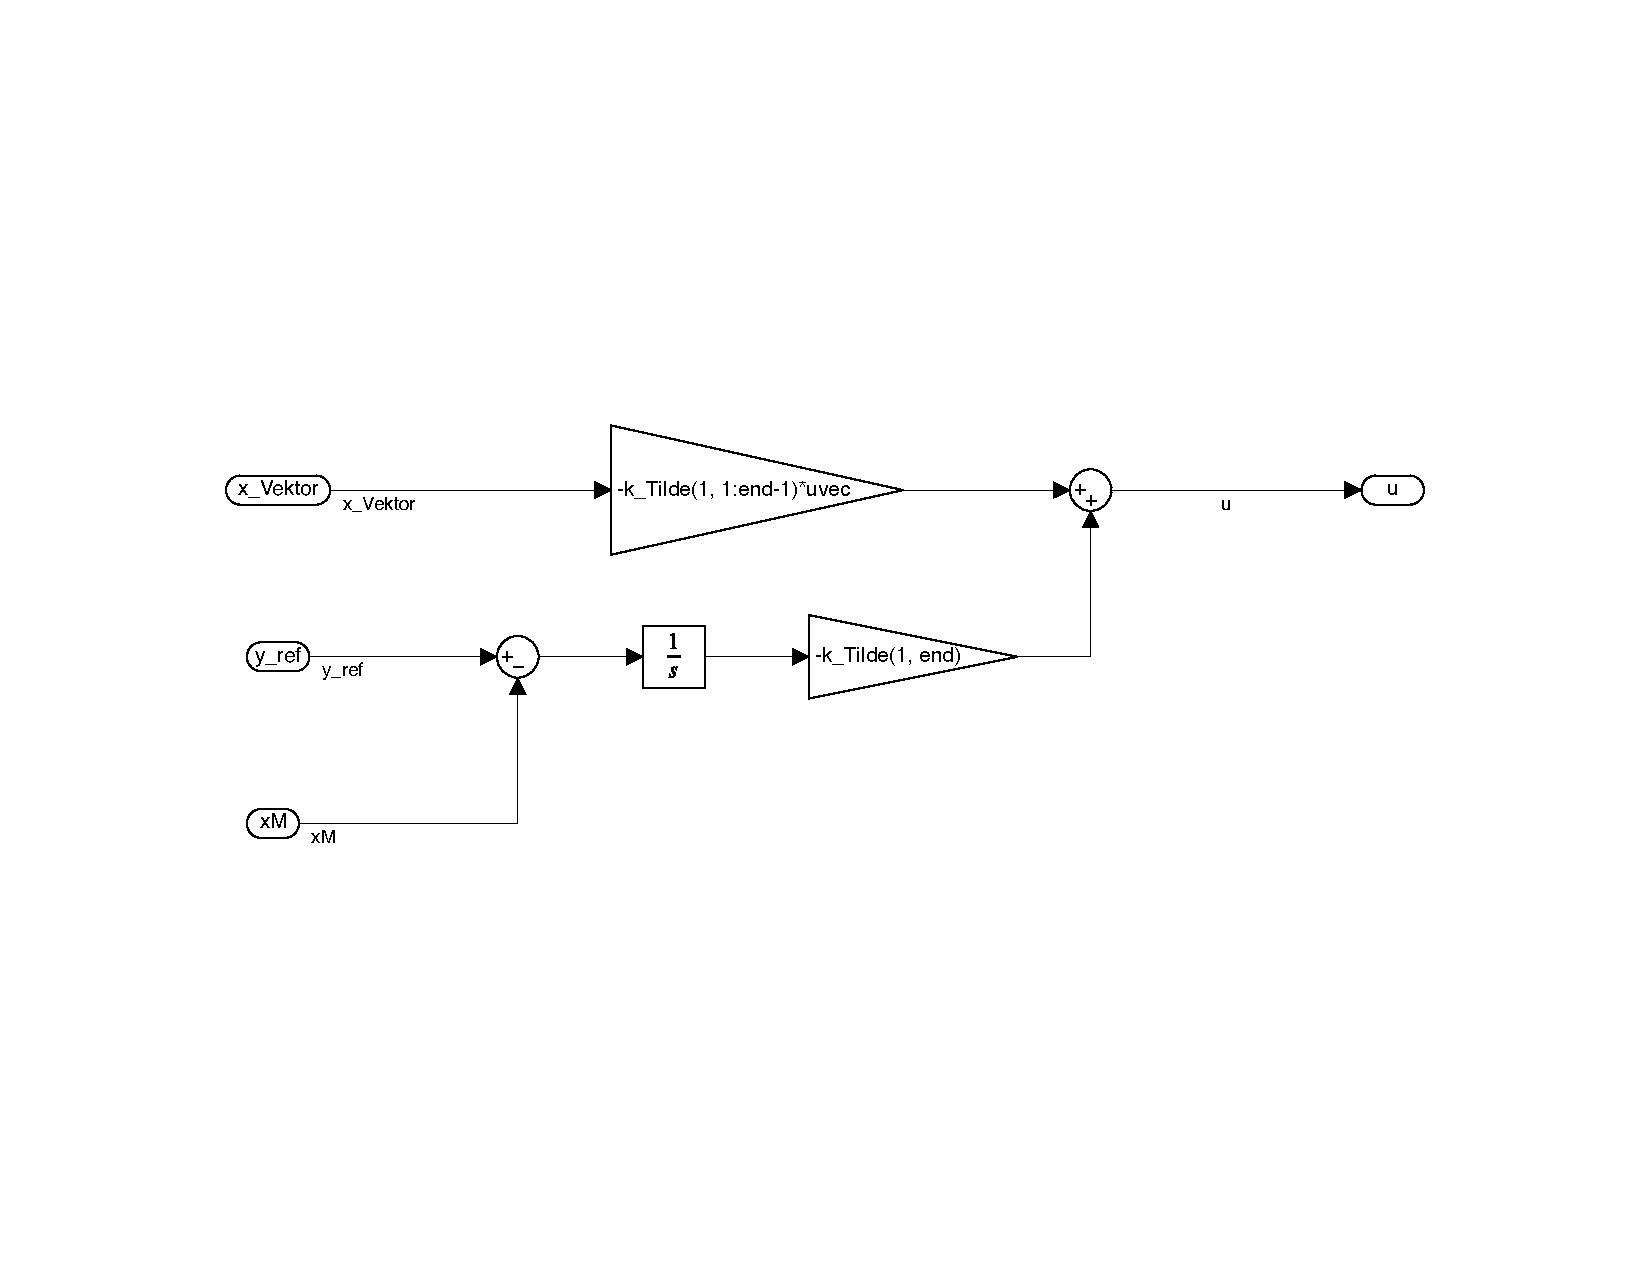
\includegraphics[width=1.0\textwidth]{Bilder/Reglervalidierung/I_Regler.pdf}}
    \caption[Regler mit I-Regelung Simulink (linear)]{Simulink Regler-Blockschaltbild für den Zustandsregler mit I-Regelung (lineares Zustandsraummodell)}
    \label{fig:Bild21}
\end{figure}

Die für die nachfolgend gezeigten Diagramme gewählten Reglerpolstellen sind in \autoref{eq:Gleichung67} gezeigt. \\
\newline
\autoref{fig:Bild22} bestätigt analog zu den vorangegangenen Reglern, dass der I-Regler wie definiert eine Anfangsauslenkung zu $0^\circ$ (obere Ruhelage) ausregeln kann. Der Winkel ist nach \ca 2,5 s wieder in der Ruhelage angelangt. \\
\newline
Das Verhalten des Wagens ist gezeigt in \autoref{fig:Bild23}. Zu erkennen ist, dass je nach vorgegebenem Referenzwert die jeweilige Referenzposition am Ende des Regelvorgangs erreicht wird. Der Vorgang braucht jedoch merklich länger mit rund 3,5 s. \\
\newline
Das dritte Diagramm (\autoref{fig:Bild24}) zeigt die benötigte Kraft des Motors, um den Wagen an die zuvor gezeigte Position zu bewegen. Zu erkennen ist, dass für größere Referenzpositionen bei großen Winkeln eine kleinere Eingangskraft benötigt wird. Dafür steigt jedoch bei kleinen Anfangsauslenkungen und großen Referenzwerten die benötigte Eingangskraft. In diesem Fall jedoch mit einem negativen Vorzeichen. Zuletzt ist festzuhalten, dass bereits nach rund 1,25 s der Motor keine Kraft mehr liefern muss.\\
\newline
Zusammenfassend kann bestätigt werden, dass sich der Regler für die deutlich weiter rechts positionierten Polstellen immer noch erwartungsgemäß verhält und die Grenzen der Anlage bezüglich maximaler Position und Kraft nicht überschritten werden.

\begin{figure}[H]
    \centering
    \fbox{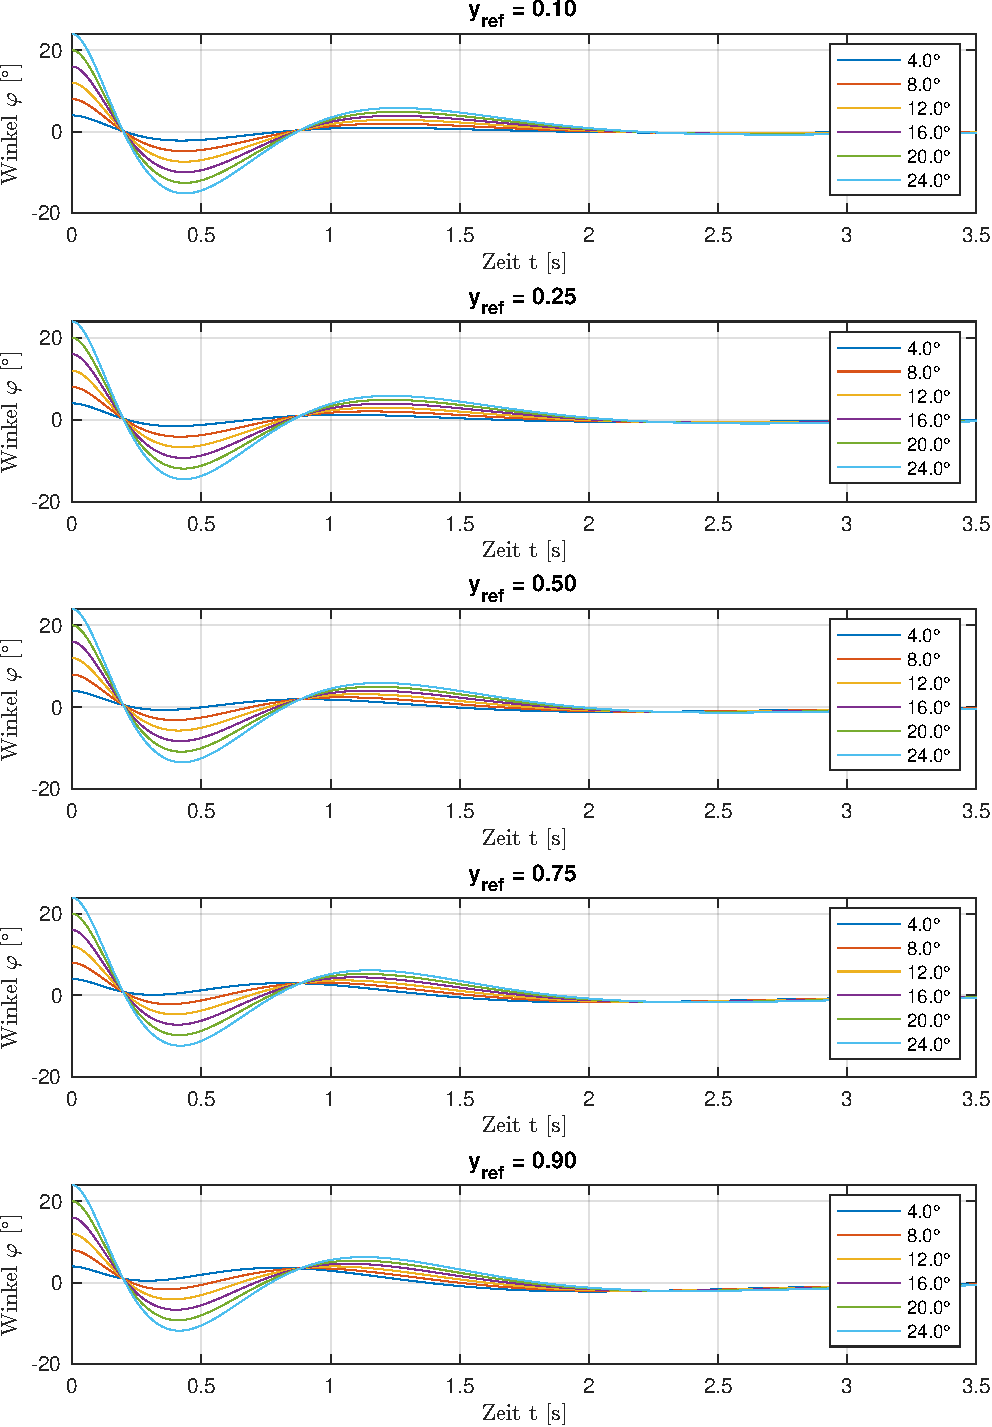
\includegraphics[width=0.76\textwidth]{Bilder/Reglervalidierung/linear_i_regler_phi.pdf}}
    \caption[$\varphi$ für Regler mit I-Regelung (linear)]{$\varphi$ für verschiedene Referenzpositionen $y_{ref}$ und Anfangsauslenkungen am Zustandsregler mit I-Regelung für das lineare Zustandsraummodell}
    \label{fig:Bild22}
\end{figure}

\begin{figure}[H]
    \centering
    \fbox{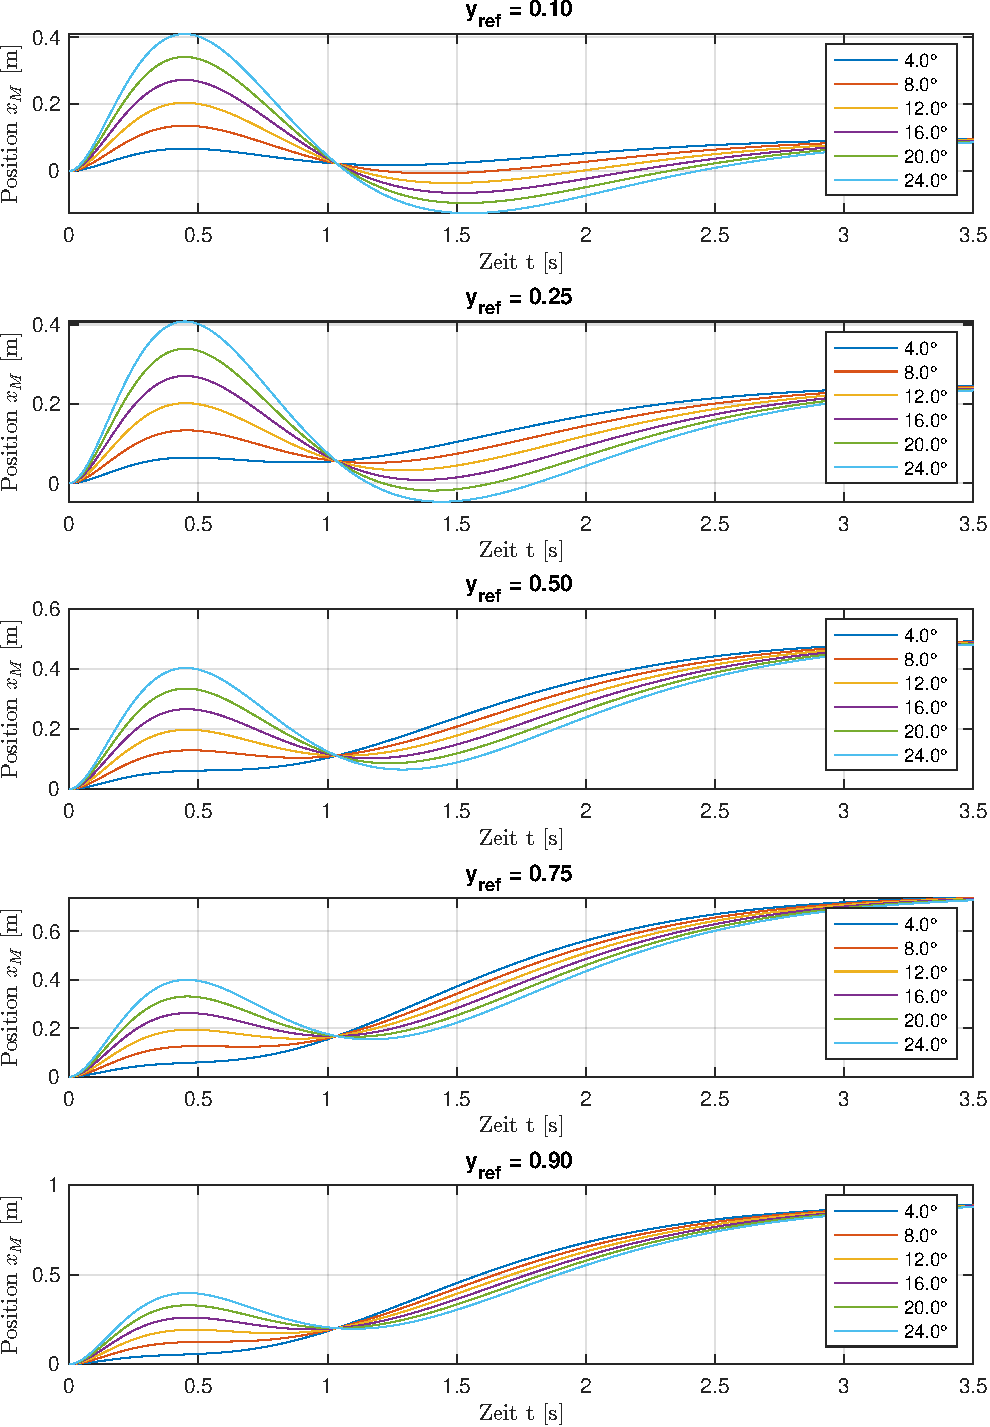
\includegraphics[width=0.76\textwidth]{Bilder/Reglervalidierung/linear_i_regler_xM.pdf}}
    \caption[$x_{\mathrm{M}}$ für Regler mit I-Regelung (linear)]{$x_{\mathrm{M}}$ für verschiedene Referenzpositionen $y_{ref}$ und Anfangsauslenkungen am Zustandsregler mit I-Regelung für das lineare Zustandsraummodell}
    \label{fig:Bild23}
\end{figure}

\begin{figure}[H]
    \centering
    \fbox{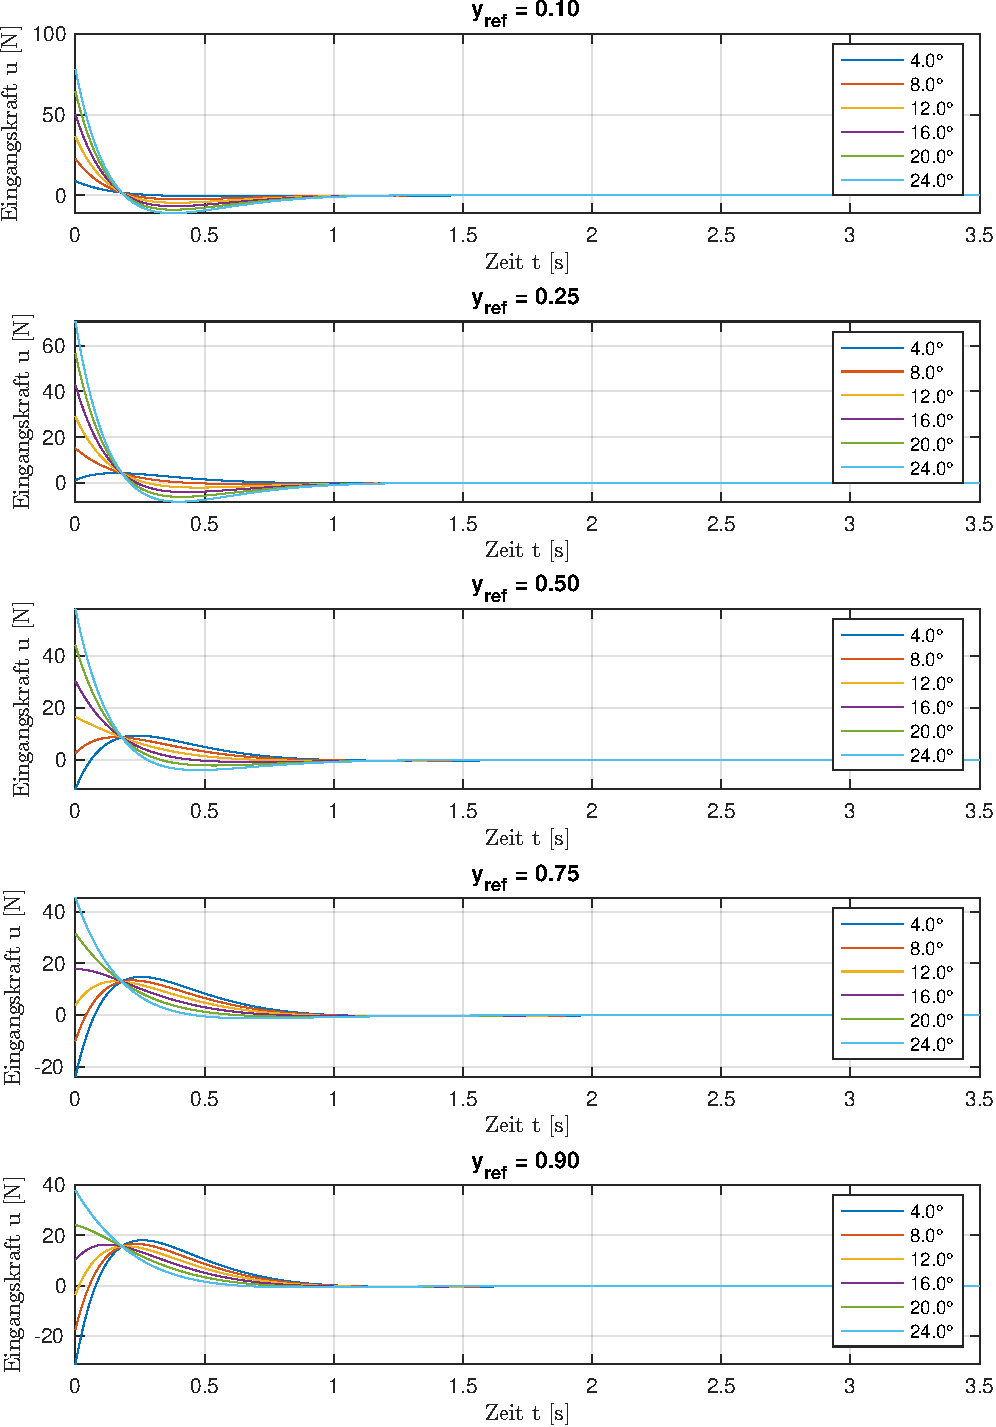
\includegraphics[width=0.76\textwidth]{Bilder/Reglervalidierung/linear_i_regler_u.pdf}}
    \caption[u für Regler mit I-Regelung (linear)]{u für verschiedene Referenzpositionen $y_{ref}$ und Anfangsauslenkungen am Zustandsregler mit I-Regelung für das lineare Zustandsraummodell}
    \label{fig:Bild24}
\end{figure}

\subsubsection{Vergleich des Regelverhaltens}

Im folgenden werden die drei implementierten Regelstrategien verglichen. Dabei soll herausgearbeitet werden, welche Vorteile für einen bestimmten Regler sprechen und welcher am geeignetsten für die Regelaufgabe ist. \\
Um eine gewisse Vergleichbarkeit sicherzustellen, wurden alle drei Simulink-Modelle der Regler inklusive Regelstrecke mit der gleichen Anfangsauslenkung simuliert. Weiterhin wurde auch die selbe Referenzposition beim Zustandsregler mit Vorsteuerung und beim Regler mit I-Regelung genutzt. \\
In Diagrammform werden nachfolgend der Winkel des Pendels $\varphi$, die Wagenposition $x_{\mathrm{M}}$ und die benötigte Eingangskraft $u$ \bzw $F_{\mathrm{a}}$ für die drei Zustandsregler dargestellt. \\
Es ist wichtig die gewählten Polstellen für den jeweiligen Regler zu berücksichtigen und diese mit in den Vergleich einzubeziehen. Nachfolgen sind die Polstellen aufgeführt:

\begin{align*}
    \underline{s}_{\mathrm{P}_{Acker.}} &= 
    \begin{bmatrix}
        -4.0 & -4.0 & -4.0 & -4.0 
    \end{bmatrix} \\
    \underline{s}_{\mathrm{P}_{Vorst.}} &= 
    \begin{bmatrix}
        -4.5 & -4.5 & -4.5 & -4.5 
    \end{bmatrix} \\
    \underline{s}_{\mathrm{P}_{I-Reg.}} &= 
    \begin{bmatrix}
        -3.2 & -3.2 & -3.2 & -3.2 
    \end{bmatrix}
\end{align*}

Die Wahl der Polstellen beruht auf der Optimierung der der Regelgeschwindigkeit bei maximalem Ausreizen der Systemgrenzen.

\begin{figure}[H]
    \centering
    \fbox{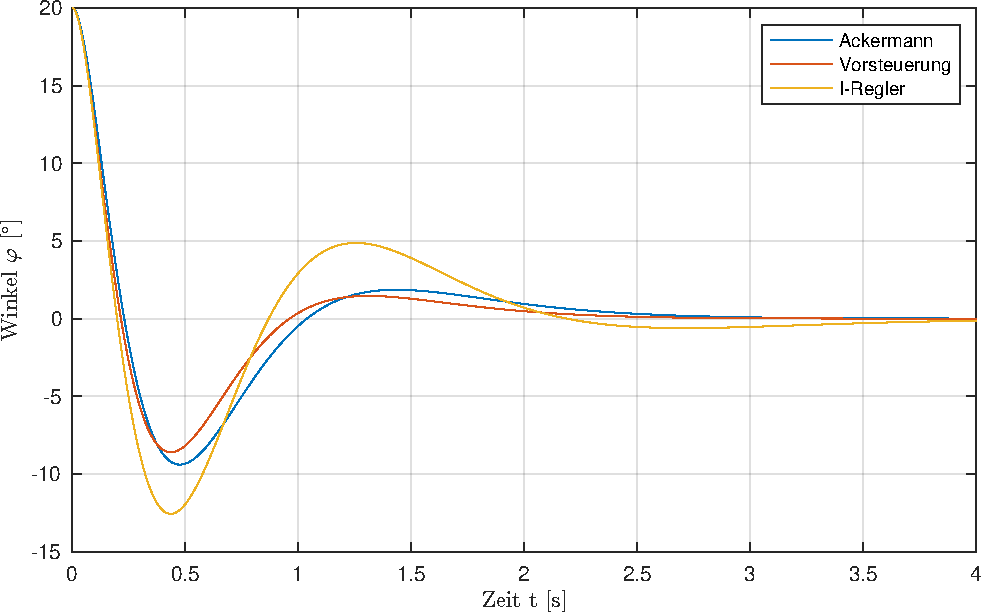
\includegraphics[width=0.65\textwidth]{Bilder/Reglervalidierung/linear_vergleich_phi.pdf}}
    \caption[Reglervergleich für $\varphi$ (linear)]{$\varphi$ für Regler mit einfacher Zustandsrückführung, Regler mit Vorsteuerung und Regler mit I-Regelung bei einer Anfangsauslenkungen von $20^\circ$ und einer Referenzposition $y_{ref} = 0,1 m$ am linearen Zustandsraummodell}
    \label{fig:Bild25}
\end{figure}

\begin{figure}[H]
    \centering
    \fbox{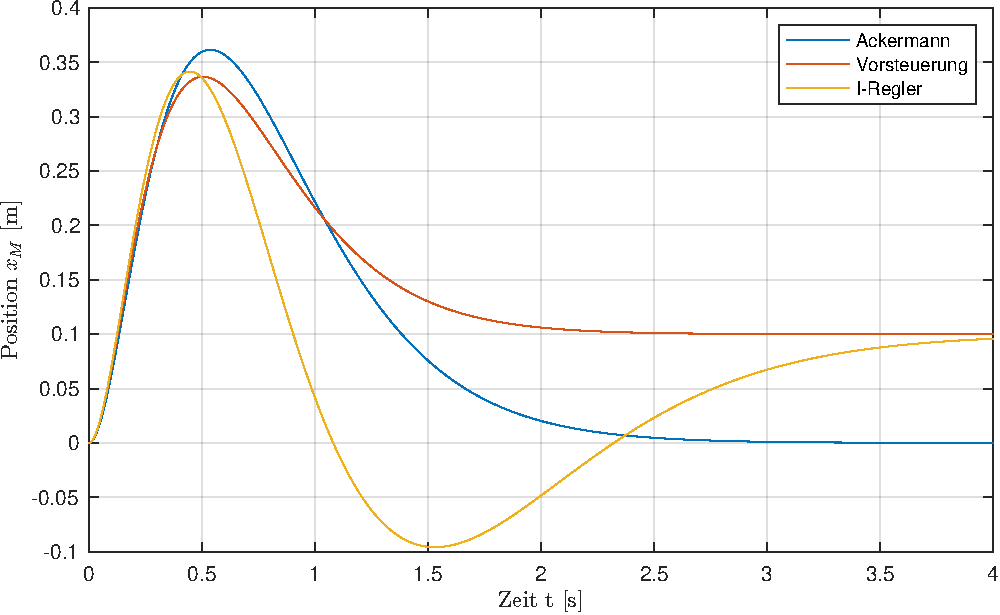
\includegraphics[width=0.65\textwidth]{Bilder/Reglervalidierung/linear_vergleich_xM.pdf}}
    \caption[Reglervergleich für $x_{\mathrm{M}}$ (linear)]{$x_{\mathrm{M}}$ für Regler mit einfacher Zustandsrückführung, Regler mit Vorsteuerung und Regler mit I-Regelung bei einer Anfangsauslenkungen von $20^\circ$ und einer Referenzposition $y_{ref} = 0,1 m$ am linearen Zustandsraummodell}
    \label{fig:Bild26}
\end{figure}

\begin{figure}[H]
    \centering
    \fbox{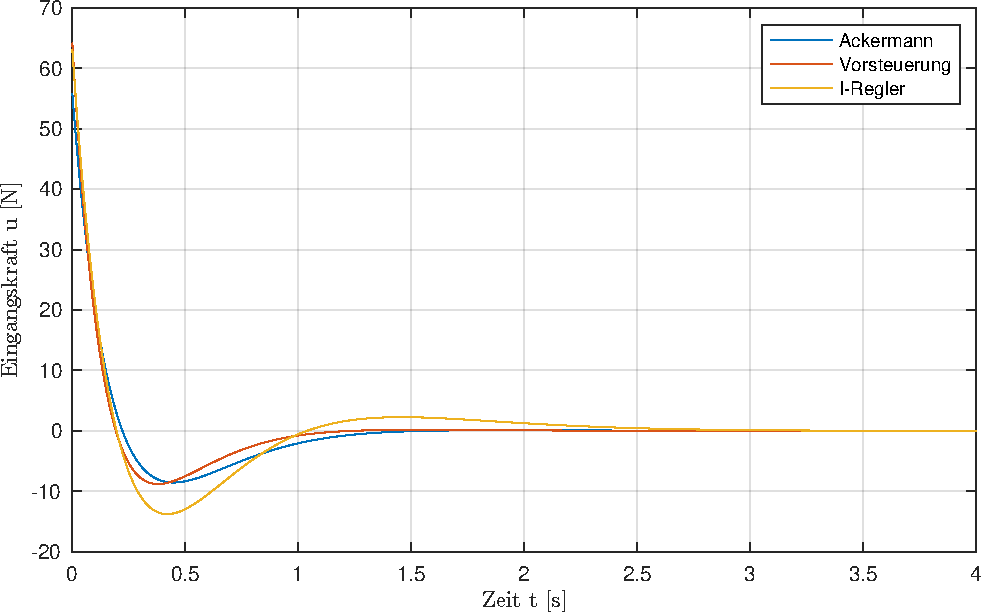
\includegraphics[width=0.65\textwidth]{Bilder/Reglervalidierung/linear_vergleich_u.pdf}}
    \caption[Reglervergleich für $u$ (linear)]{$u$ für Regler mit einfacher Zustandsrückführung, Regler mit Vorsteuerung und Regler mit I-Regelung bei einer Anfangsauslenkungen von $20^\circ$ und einer Referenzposition $y_{ref} = 0,1 m$ am linearen Zustandsraummodell}
    \label{fig:Bild27}
\end{figure}

\autoref{fig:Bild25} zeigt, dass der Winkel des Pendels bei der Regelung mit Vorsteuerung für die oben gewählten Polstellen am schnellsten wieder in der Ruhelage ausgeregelt ist. Dieses Verhalten lässt sich dadurch begründen, dass die Polstellen bei der Vorsteuerung etwas weiter nach links gelegt wurden im Vergleich zum Regler mit einfacher Zustandsrückführung (Ackermann), wodurch der Regler schneller wird. Grundsätzlich würden die Kurvenverläufe der beiden genannten Regler annähernd identisch sein, wenn die Polstellen die gleichen sind und bei der Vorsteuerung die Referenzposition zu Null gewählt wird. Verschiebt man bei positiver Anfangsauslenkung jedoch die Referenzposition nach rechts, so würde der Regler mit Vorsteuerung deutlich schneller wieder in die Ruhelage regeln, da er nicht dafür sorgen muss, dass der Wagen wieder auf der Nullposition stehen bleibt. Der Zustandsregler mit I-Regelung scheint im Gegensatz generell etwas langsamer zu sein, selbst wenn die Polstellen für alle Regelstrategien gleich gewählt werden. \\
Weiterhin ist zu erkennen, das bei der I-Regelung ein stärkeres Schwingen auftritt, welches durch das Aufintegrieren des Regelfehlers zu erklären ist. \\
\newline
In \autoref{fig:Bild26} ist vor allem der wesentliche Unterschied zwischen dem Regler mit einfacher Zustandsrückführung und den Reglern mit Zustandsrückführung und Referenzwertvorgabe zu erkennen. Bei der Vorsteuerung und I-Regelung kann in den jeweiligen Graphen die gewählte Referenzposition am rechten Ende des Diagramms abgelesen werden. Der Zustandsregler mit Ackermann-Formel regelt die Wagenposition wieder auf Null zurück. \\
Auch hier kann das stärkere Schwingverhalten des I-Reglers identifiziert werden. \\
\newline
Der wesentliche Grund für die Wahl der Polstellen wird in \autoref{fig:Bild27} ersichtlich. Für eine einheitliche Auslenkung des Pendels ist die Eingangskraft $u$ annähernd gleich bei den drei Reglern. Für die in den vorangegangenen Unterabschnitten ermittelten maximalen Auslenkungen ist die Eingangskraft $u$ \bzw $F_{\mathrm{a}}$ im Maximum knapp unter 80 N groß. Somit wird das System bei den gewählten Polstellen maximal ausgereizt. \\
Wie auch schon bei der Betrachtung des Winkels $\varphi$ und der Wagenposition $x_{\mathrm{M}}$ kann ein stärkeres Schwingungsverhalten beim Zustandsregler mit I-Regelung erkannt werden.

\newpage

\subsection{Validierung des nicht-linearen Modells}
Im folgenden werden die drei Regler für das nicht-lineare Zustandsraummodell validiert. Die Simulink Implementierung der nicht-linearen Regelstrecke ist in \autoref{fig:Bild2} dargestellt. \\
\newline
Wie im vorangegangenen Unterabschnitt werden Diagramme für den Winkel des Pendels $\varphi$, die Wagenposition $x_{\mathrm{M}}$ und die benötigte Eingangskraft $u$ \bzw $F_{\mathrm{a}}$ für die drei Zustandsregler gezeigt. Es wird jedoch auf Kommentare verzichtet, da die Anwendung der Regler auf das nicht-lineare Zustandsraummodell zu analogen Ergebnissen führt, was bereits in \autoref{sec:systemvergleich} nachgewiesen wurde.

\subsubsection{Zustandsregler mit einfacher Rückführung}

\begin{figure}[H]
    \centering
    \fbox{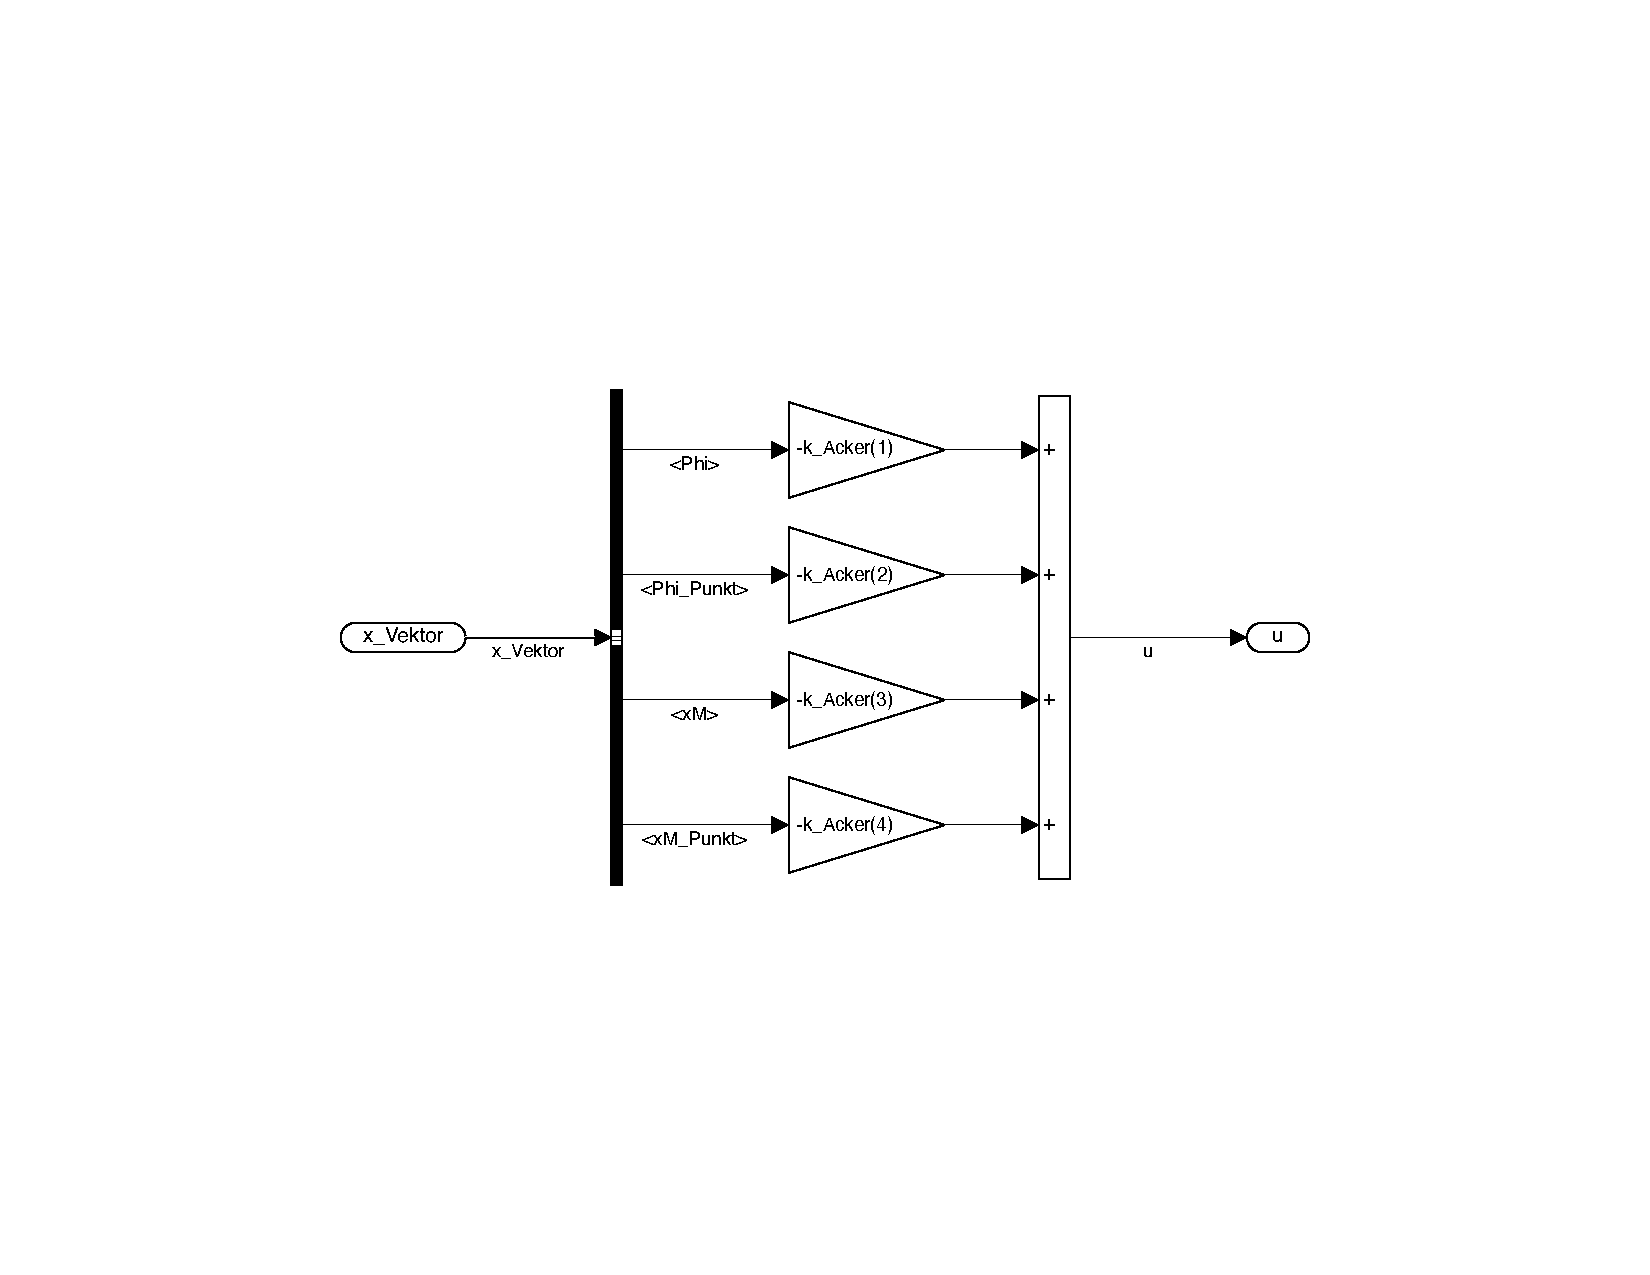
\includegraphics[width=1.0\textwidth]{Bilder/Reglervalidierung/Ackermann_Regler_nl.pdf}}
    \caption[Zustandsregler mit einfacher Rückführung - Simulink (nicht-linear)]{Simulink Regler-Blockschaltbild für den Zustandsregler mit einfacher Zustandsrückführung (nicht-lineares Zustandsraummodell)}
    \label{fig:Bild28}
\end{figure}

\begin{figure}[H]
    \centering
    \fbox{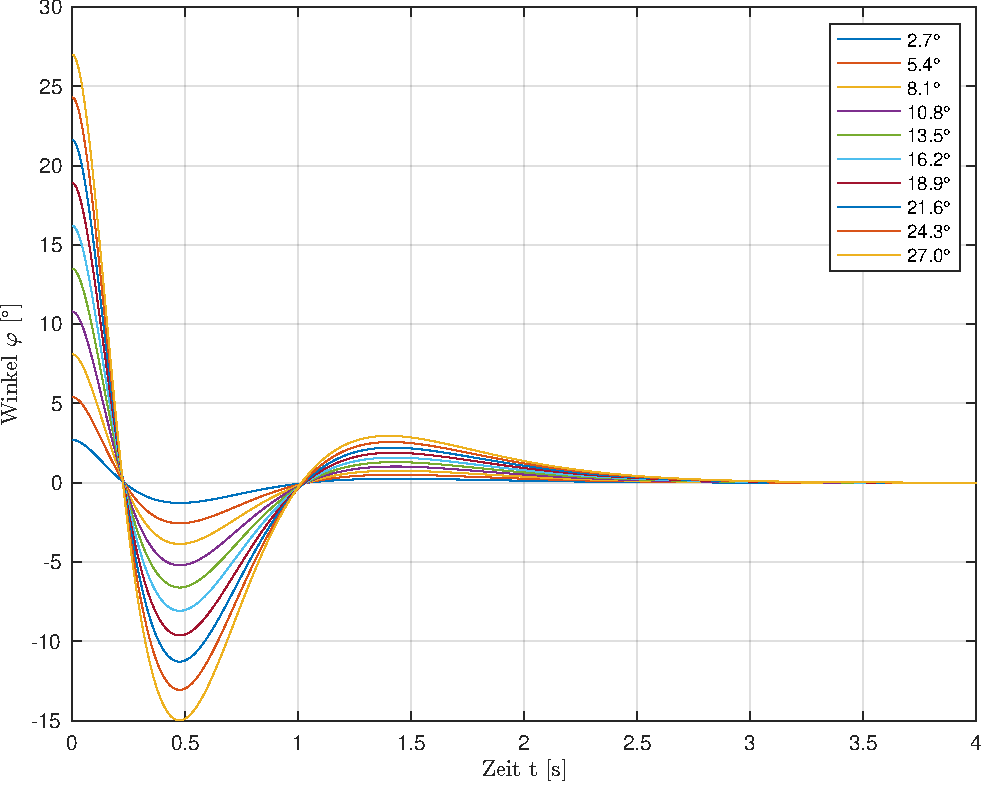
\includegraphics[width=0.6\textwidth]{Bilder/Reglervalidierung/nichtlinear_ackermann_phi.pdf}}
    \caption[$\varphi$ für Regler mit einfacher Rückführung (nicht-linear)]{$\varphi$ für verschiedene Anfangsauslenkungen am Zustandsregler mit einfacher Rückführung für das nicht-lineare Zustandsraummodell}
    \label{fig:Bild29}
\end{figure}

\begin{figure}[H]
    \centering
    \fbox{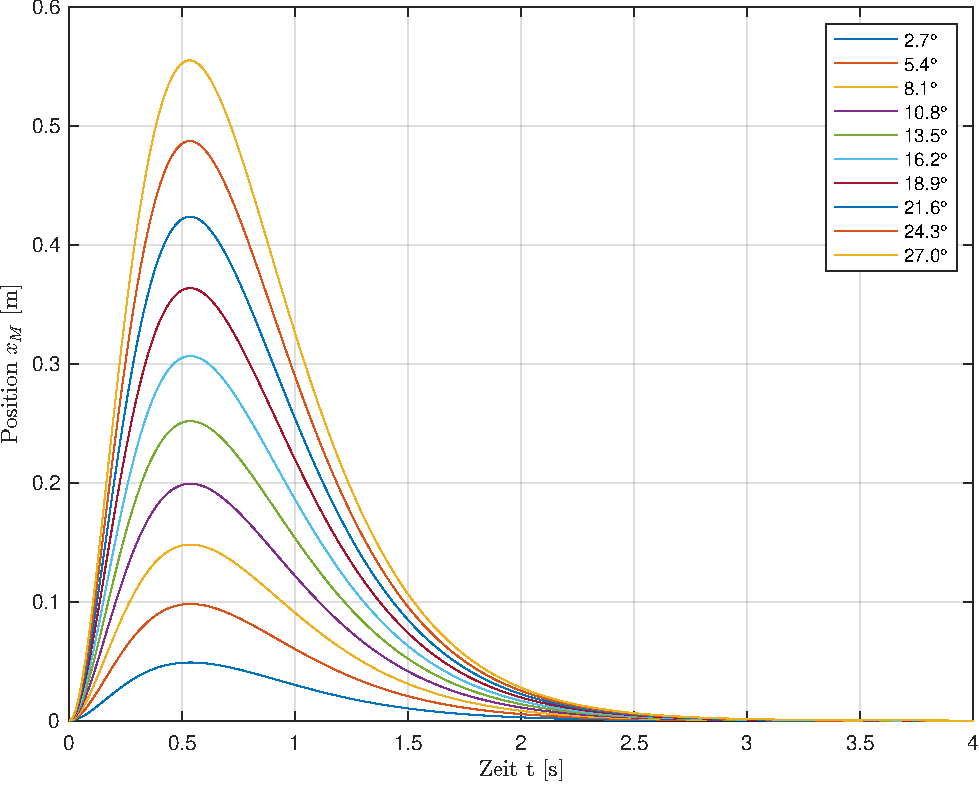
\includegraphics[width=0.6\textwidth]{Bilder/Reglervalidierung/nichtlinear_ackermann_xM.pdf}}
    \caption[$x_{\mathrm{M}}$ für Regler mit einfacher Rückführung (nicht-linear)]{$x_{\mathrm{M}}$ für verschiedene Anfangsauslenkungen am Zustandsregler mit einfacher Rückführung für das nicht-lineare Zustandsraummodell}
    \label{fig:Bild30}
\end{figure}

\begin{figure}[H]
    \centering
    \fbox{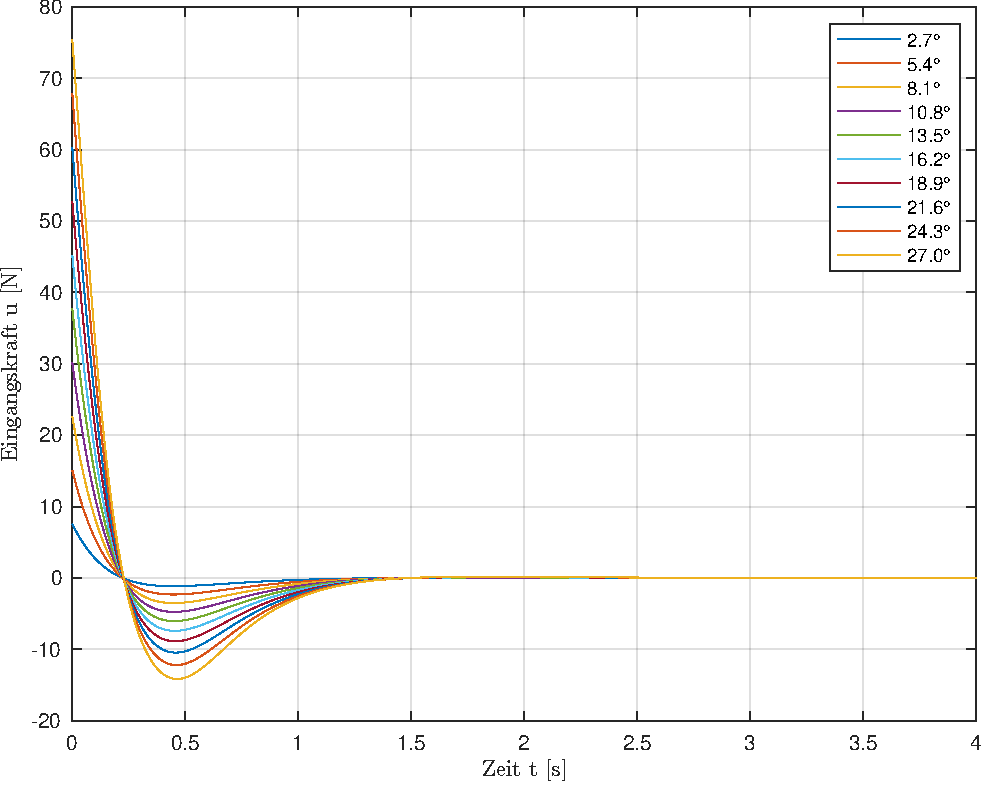
\includegraphics[width=0.6\textwidth]{Bilder/Reglervalidierung/nichtlinear_ackermann_u.pdf}}
    \caption[u für Regler mit einfacher Rückführung (nicht-linear)]{u für verschiedene Anfangsauslenkungen am Zustandsregler mit einfacher Rückführung für das nicht-lineare Zustandsraummodell}
    \label{fig:Bild31}
\end{figure}

\subsubsection{Zustandsregler mit Vorsteuerung}

\begin{figure}[H]
    \centering
    \fbox{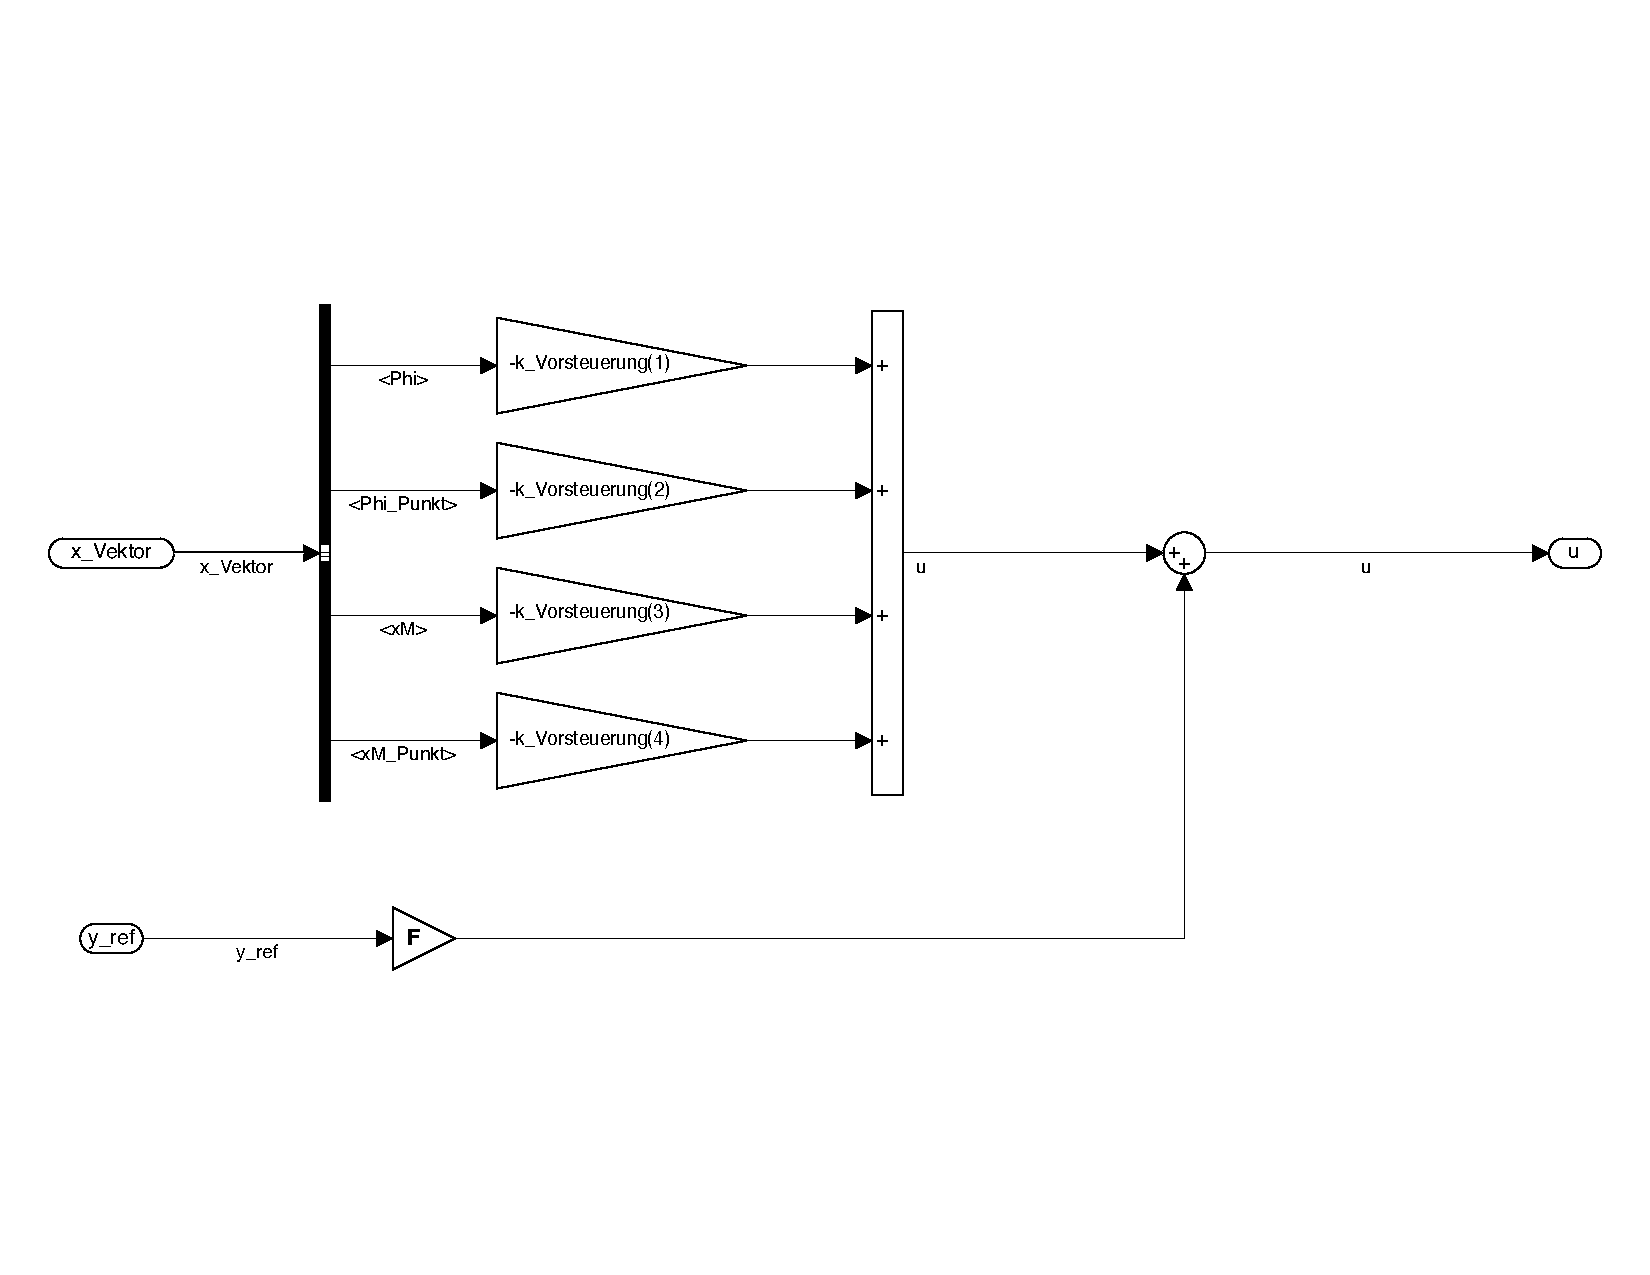
\includegraphics[width=1.0\textwidth]{Bilder/Reglervalidierung/Vorsteuerung_Regler_nl.pdf}}
    \caption[Regler mit Vorsteuerung Simulink (nicht-linear)]{Simulink Regler-Blockschaltbild für den Zustandsregler mit Vorsteuerung (nicht-lineares Zustandsraummodell)}
    \label{fig:Bild32}
\end{figure}

\begin{figure}[H]
    \centering
    \fbox{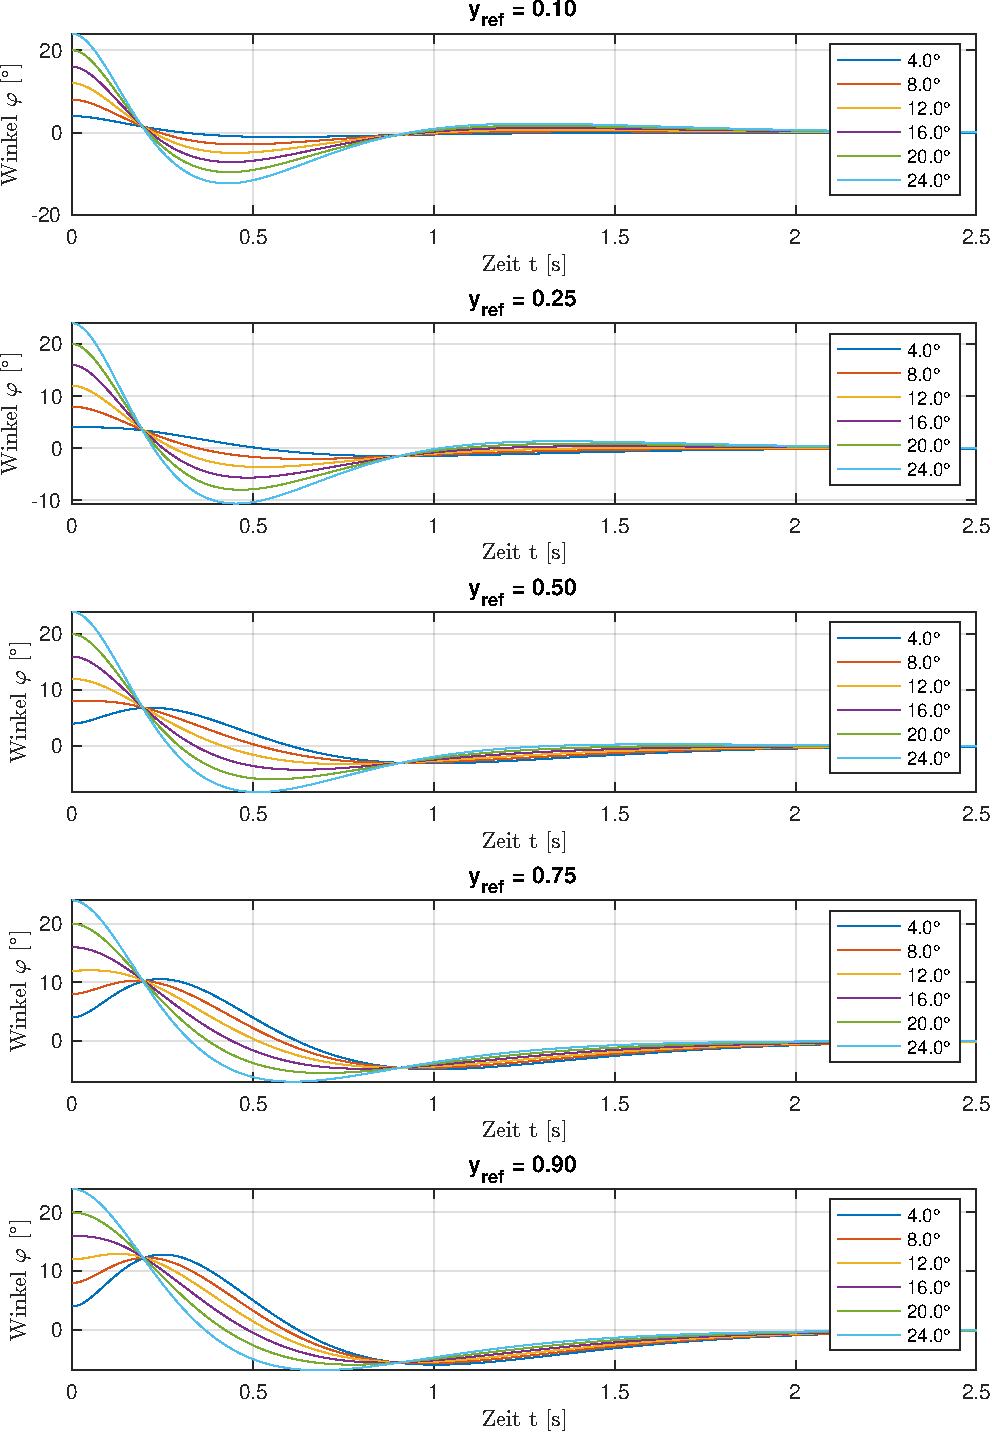
\includegraphics[width=0.76\textwidth]{Bilder/Reglervalidierung/nichtlinear_vorsteuerung_phi.pdf}}
    \caption[$\varphi$ für Regler mit Vorsteuerung (nicht-linear)]{$\varphi$ für verschiedene Referenzpositionen $y_{ref}$ und Anfangsauslenkungen am Zustandsregler mit Vorsteuerung für das nicht-lineare Zustandsraummodell}
    \label{fig:Bild33}
\end{figure}

\begin{figure}[H]
    \centering
    \fbox{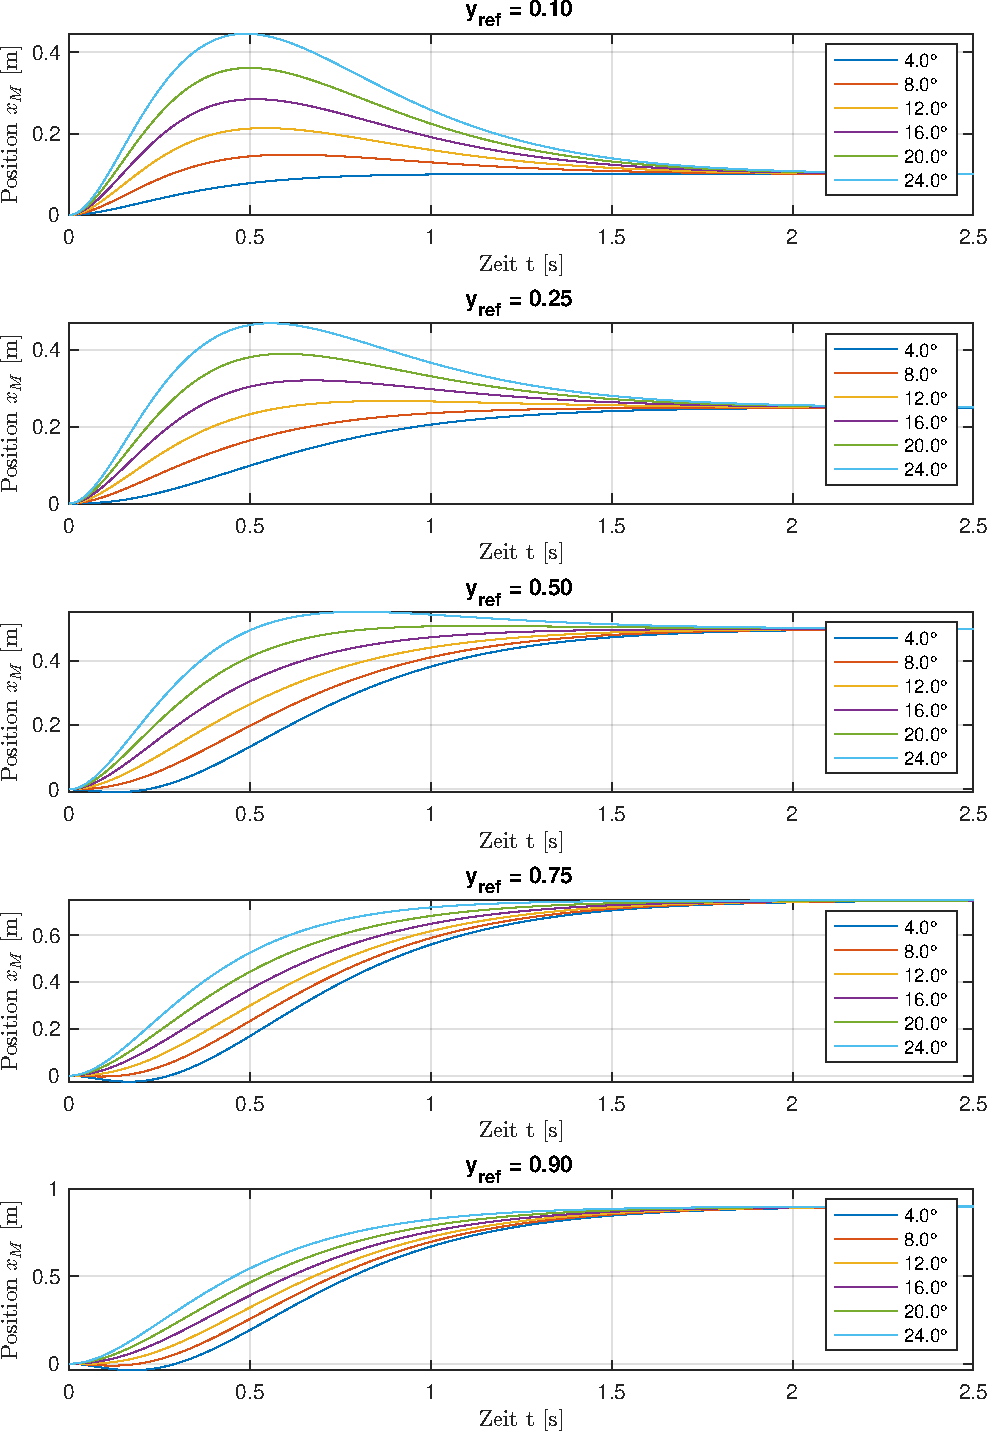
\includegraphics[width=0.76\textwidth]{Bilder/Reglervalidierung/nichtlinear_vorsteuerung_xM.pdf}}
    \caption[$x_{\mathrm{M}}$ für Regler mit Vorsteuerung (nicht-linear)]{$x_{\mathrm{M}}$ für verschiedene Referenzpositionen $y_{ref}$ und Anfangsauslenkungen am Zustandsregler mit Vorsteuerung für das nicht-lineare Zustandsraummodell}
    \label{fig:Bild34}
\end{figure}

\begin{figure}[H]
    \centering
    \fbox{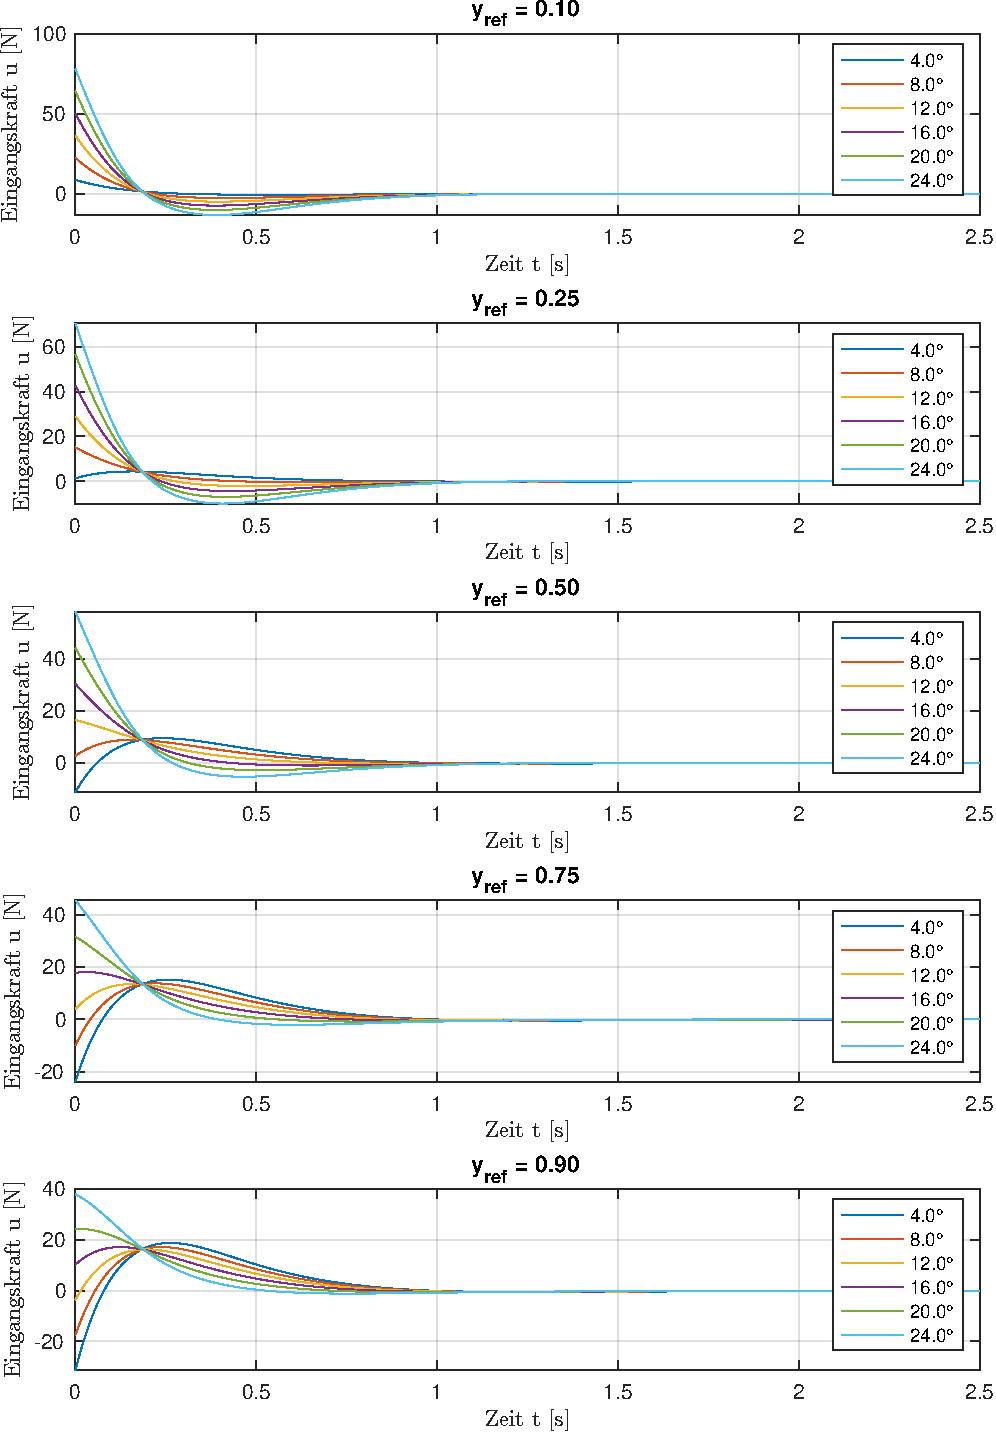
\includegraphics[width=0.76\textwidth]{Bilder/Reglervalidierung/nichtlinear_vorsteuerung_u.pdf}}
    \caption[u für Regler mit Vorsteuerung (nicht-linear)]{u für verschiedene Referenzpositionen $y_{ref}$ und Anfangsauslenkungen am Zustandsregler mit Vorsteuerung für das nicht-lineare Zustandsraummodell}
    \label{fig:Bild35}
\end{figure}

\subsubsection{Zustandsregler mit I-Regelung}

\begin{figure}[H]
    \centering
    \fbox{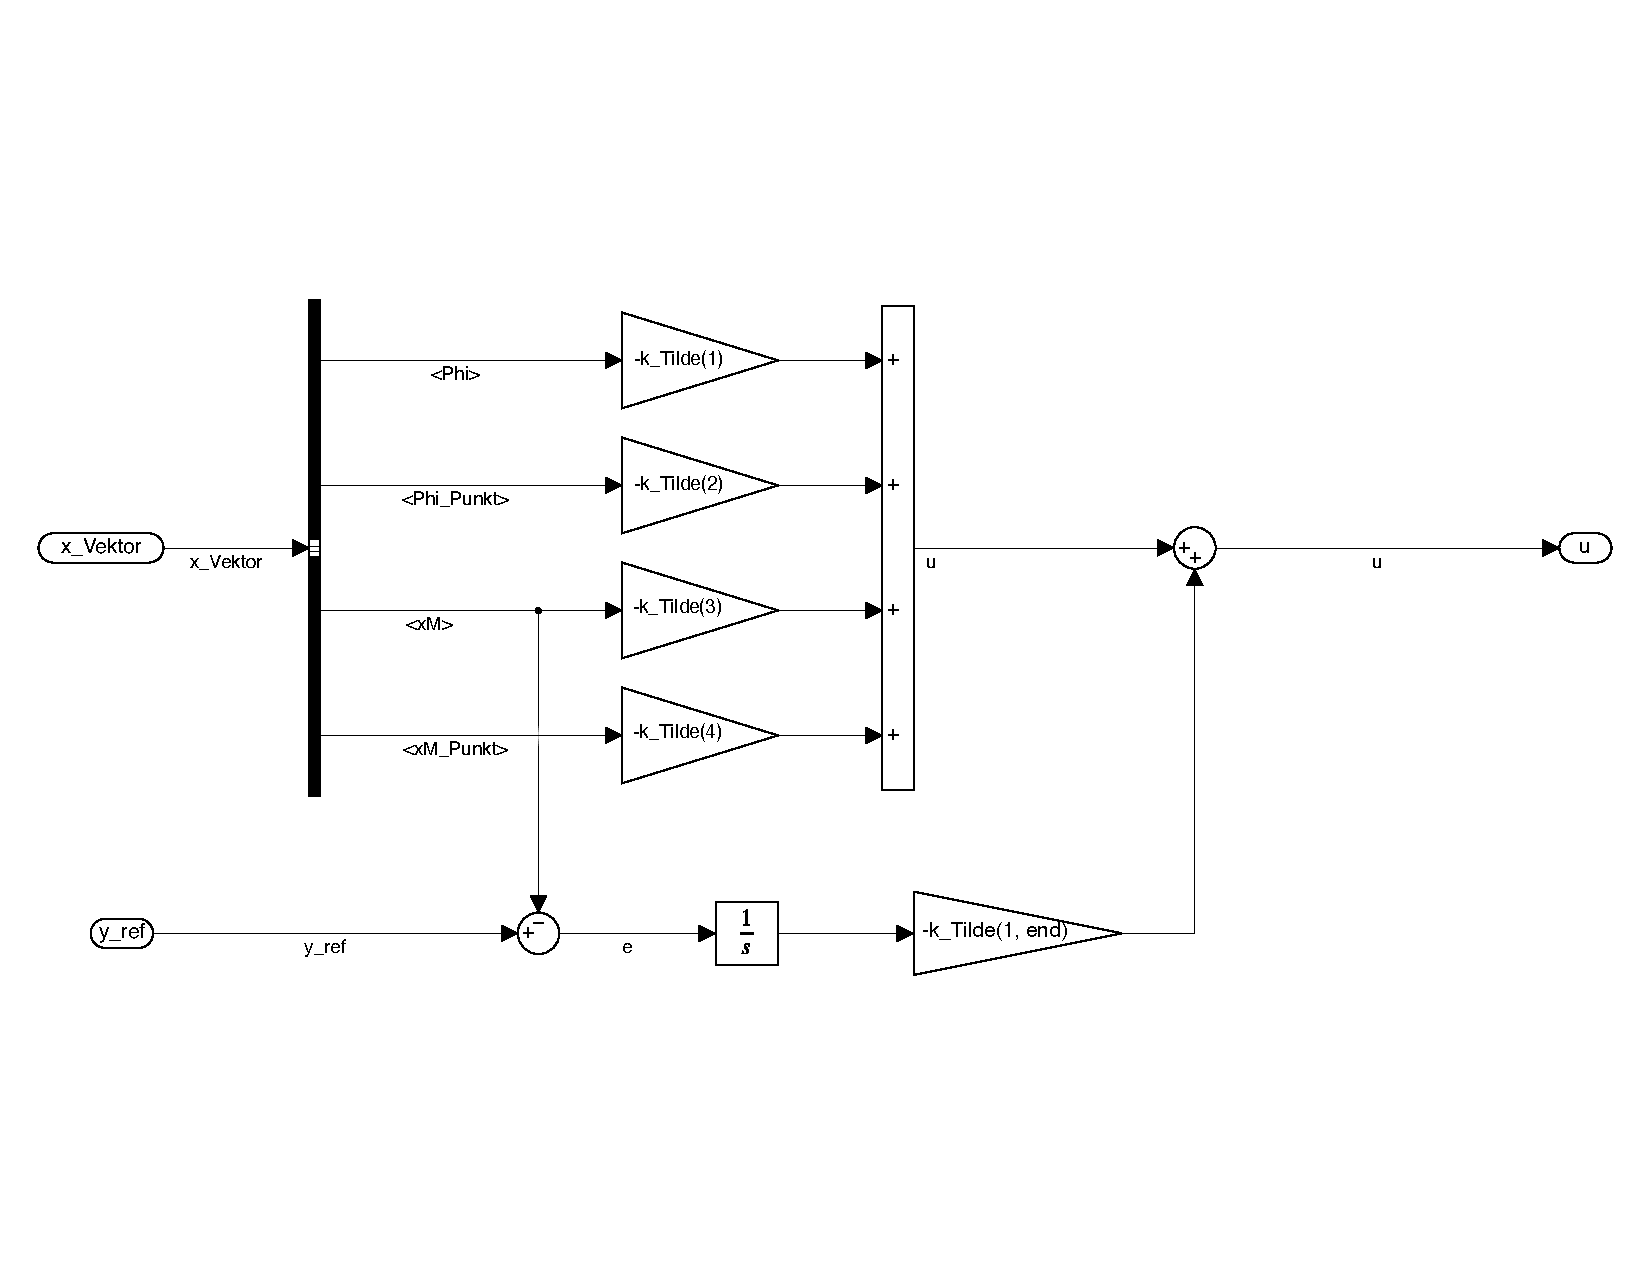
\includegraphics[width=1.0\textwidth]{Bilder/Reglervalidierung/I_Regler_nl.pdf}}
    \caption[Regler mit I-Regelung Simulink (nicht-linear)]{Simulink Regler-Blockschaltbild für den Zustandsregler mit I-Regelung (nicht-lineares Zustandsraummodell)}
    \label{fig:Bild36}
\end{figure}

\begin{figure}[H]
    \centering
    \fbox{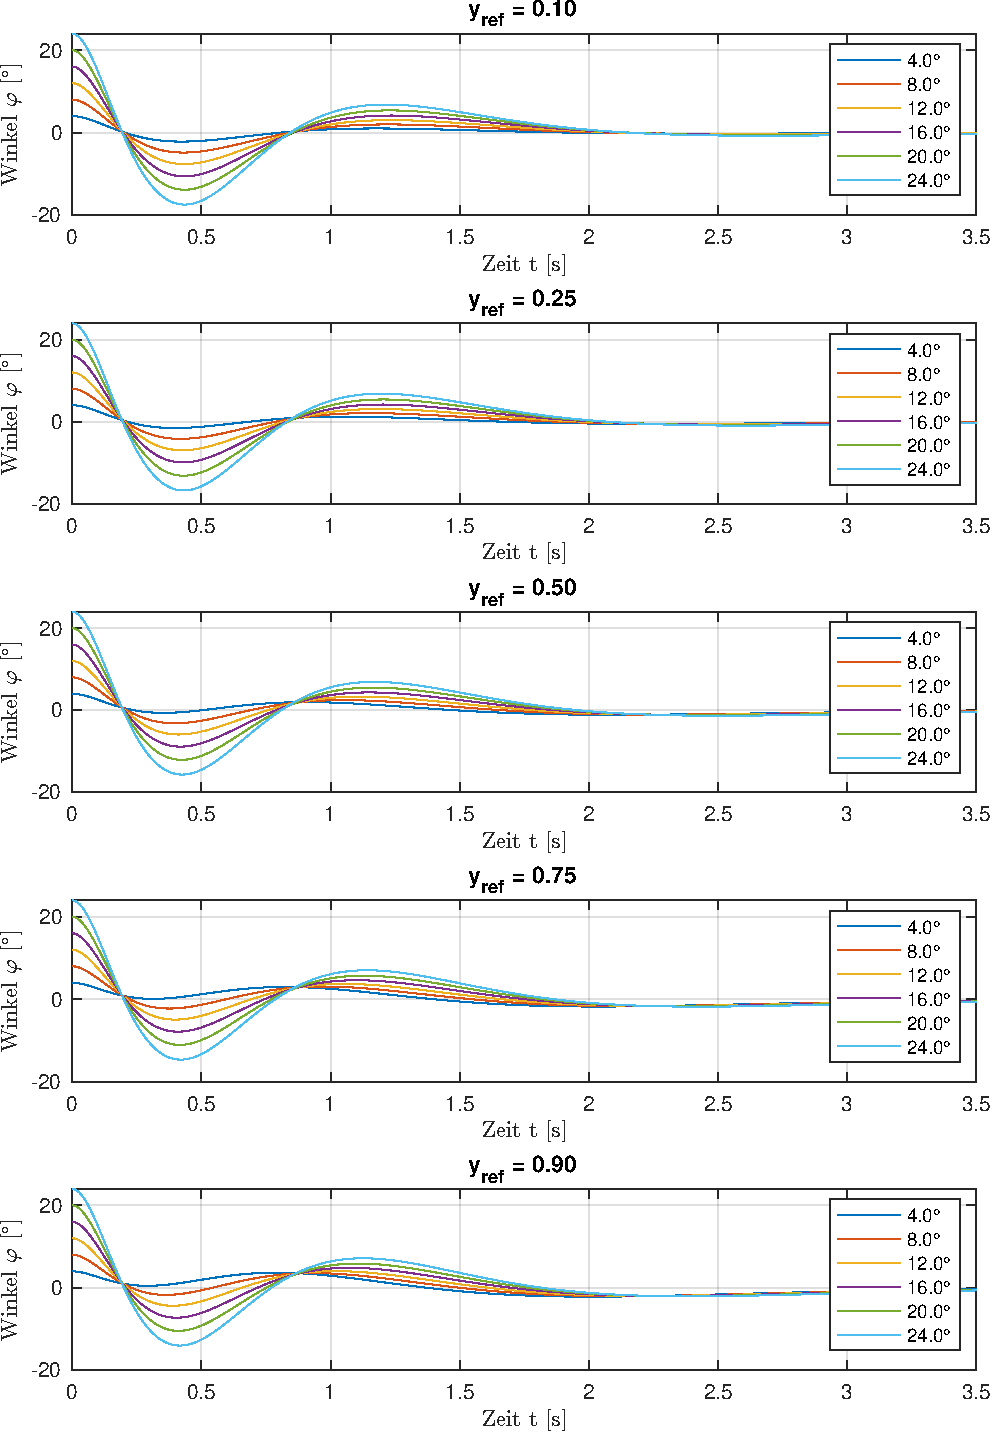
\includegraphics[width=0.76\textwidth]{Bilder/Reglervalidierung/nichtlinear_i_regler_phi.pdf}}
    \caption[$\varphi$ für Regler mit I-Regelung (nicht-linear)]{$\varphi$ für verschiedene Referenzpositionen $y_{ref}$ und Anfangsauslenkungen am Zustandsregler mit I-Regelung für das nicht-lineare Zustandsraummodell}
    \label{fig:Bild37}
\end{figure}

\begin{figure}[H]
    \centering
    \fbox{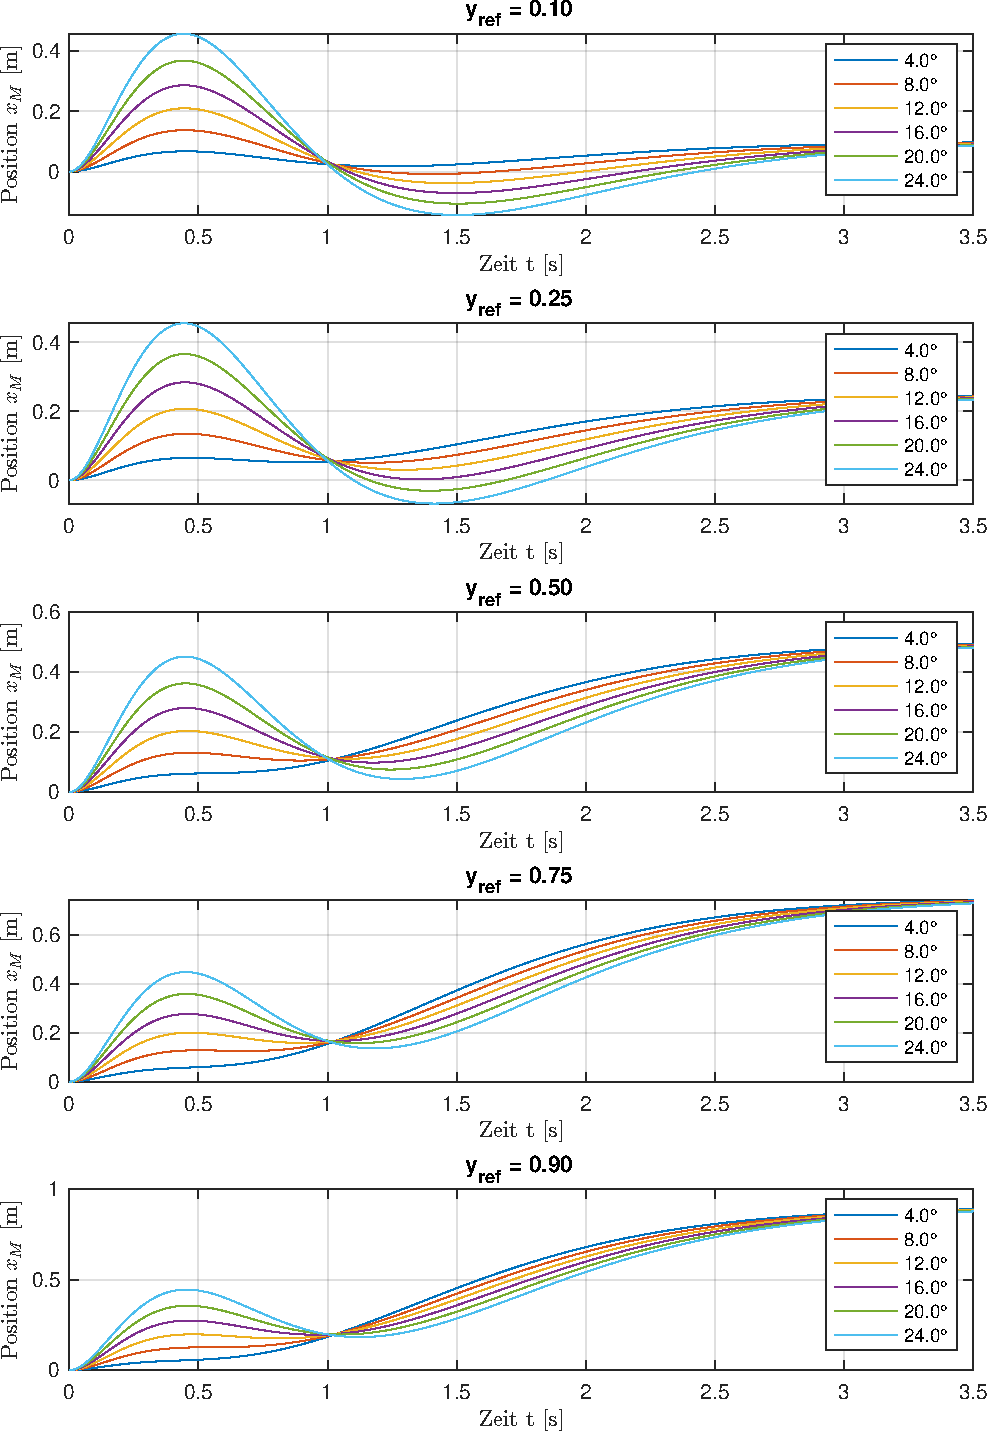
\includegraphics[width=0.76\textwidth]{Bilder/Reglervalidierung/nichtlinear_i_regler_xM.pdf}}
    \caption[$x_{\mathrm{M}}$ für Regler mit I-Regelung (nicht-linear)]{$x_{\mathrm{M}}$ für verschiedene Referenzpositionen $y_{ref}$ und Anfangsauslenkungen am Zustandsregler mit I-Regelung für das nicht-lineare Zustandsraummodell}
    \label{fig:Bild38}
\end{figure}

\begin{figure}[H]
    \centering
    \fbox{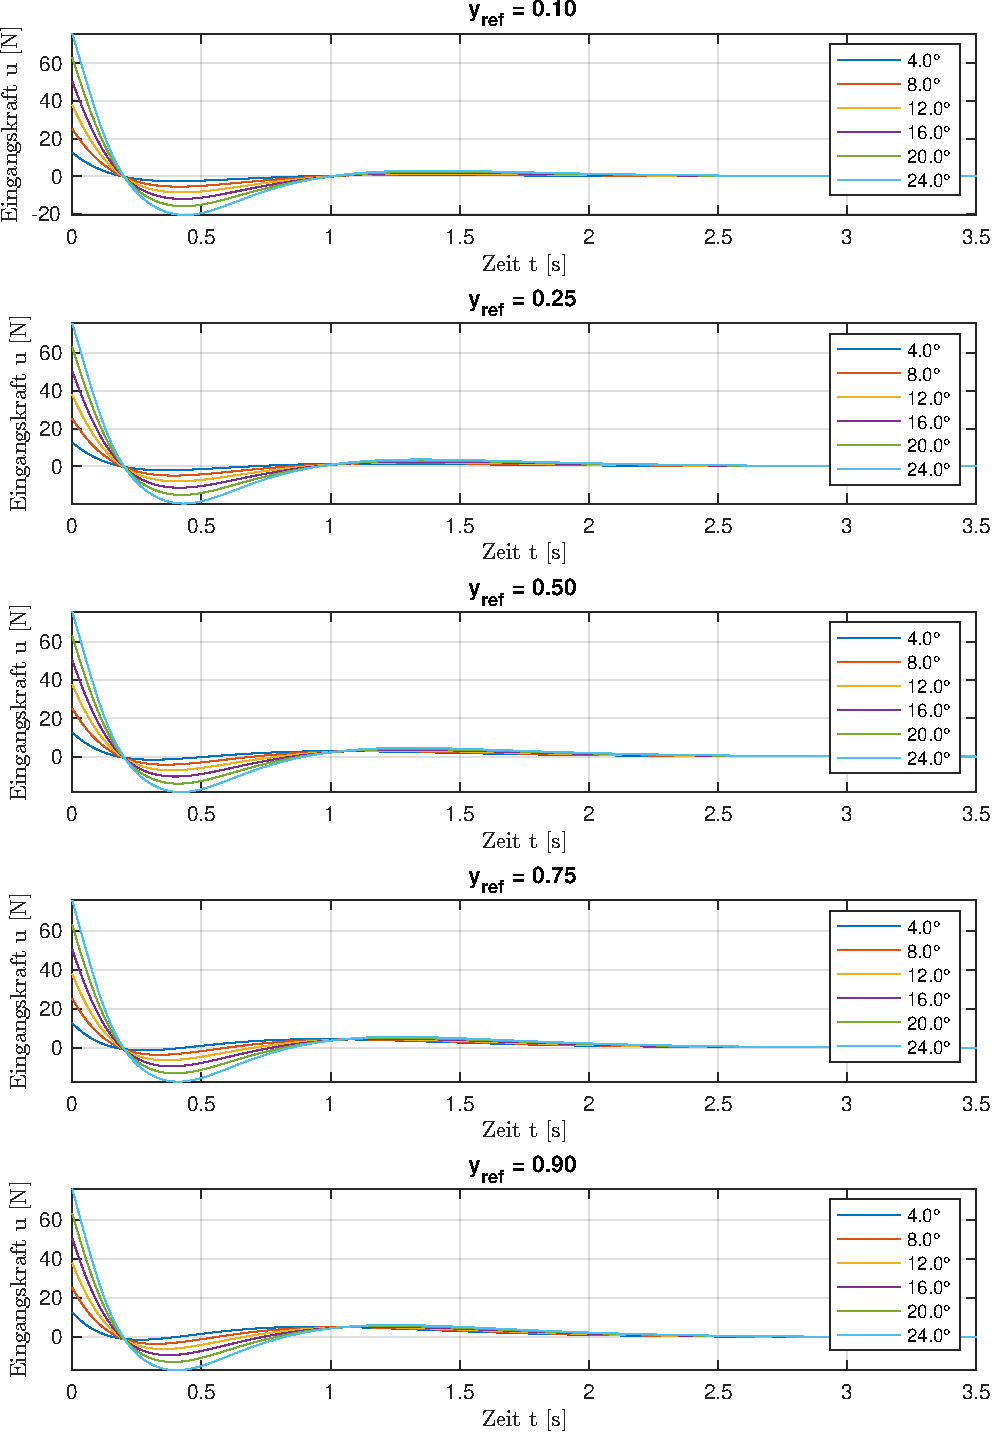
\includegraphics[width=0.76\textwidth]{Bilder/Reglervalidierung/nichtlinear_i_regler_u.pdf}}
    \caption[u für Regler mit I-Regelung (nicht-linear)]{u für verschiedene Referenzpositionen $y_{ref}$ und Anfangsauslenkungen am Zustandsregler mit I-Regelung für das nicht-lineare Zustandsraummodell}
    \label{fig:Bild39}
\end{figure}

\subsubsection{Vergleich des Regelverhaltens}

\begin{figure}[H]
    \centering
    \fbox{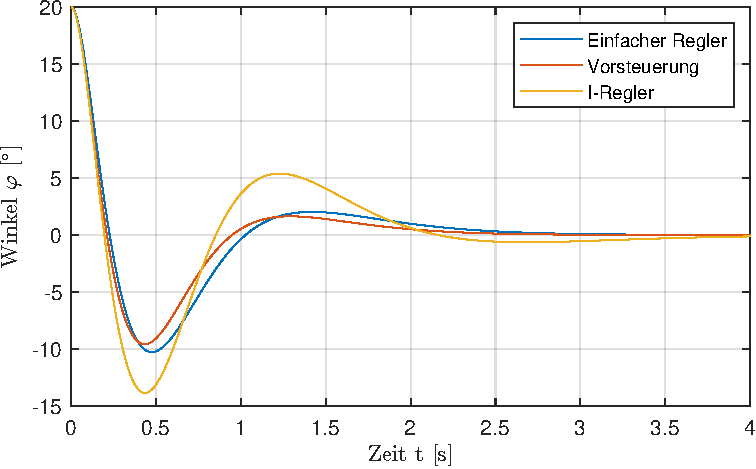
\includegraphics[width=0.65\textwidth]{Bilder/Reglervalidierung/nichtlinear_vergleich_phi.pdf}}
    \caption[Reglervergleich für $\varphi$ (nicht-linear)]{$\varphi$ für Regler mit einfacher Zustandsrückführung, Regler mit Vorsteuerung und Regler mit I-Regelung bei einer Anfangsauslenkungen von $20^\circ$ und einer Referenzposition $y_{ref} = 0,1 m$ am nicht-linearen Zustandsraummodell}
    \label{fig:Bild40}
\end{figure}

\begin{figure}[H]
    \centering
    \fbox{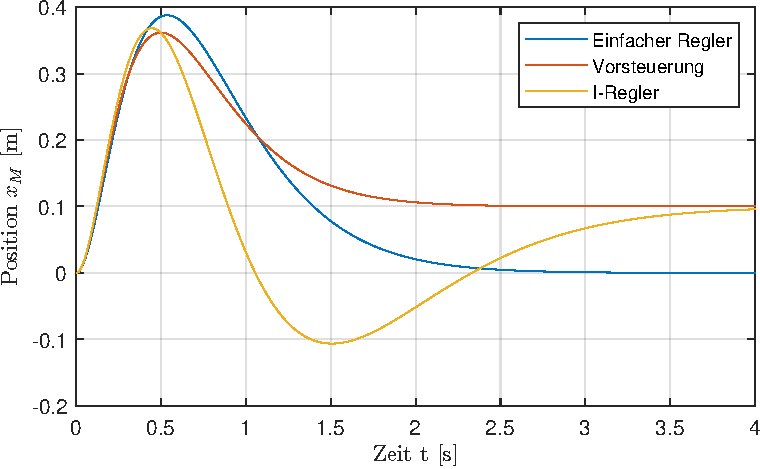
\includegraphics[width=0.65\textwidth]{Bilder/Reglervalidierung/nichtlinear_vergleich_xM.pdf}}
    \caption[Reglervergleich für $x_{\mathrm{M}}$ (nicht-linear)]{$x_{\mathrm{M}}$ für Regler mit einfacher Zustandsrückführung, Regler mit Vorsteuerung und Regler mit I-Regelung bei einer Anfangsauslenkungen von $20^\circ$ und einer Referenzposition $y_{ref} = 0,1 m$ am nicht-linearen Zustandsraummodell}
    \label{fig:Bild41}
\end{figure}

\begin{figure}[H]
    \centering
    \fbox{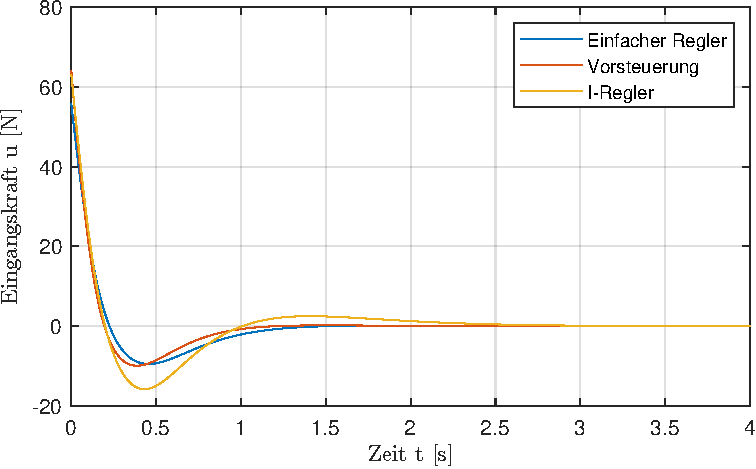
\includegraphics[width=0.65\textwidth]{Bilder/Reglervalidierung/nichtlinear_vergleich_u.pdf}}
    \caption[Reglervergleich für $u$ (nicht-linear)]{$u$ für Regler mit einfacher Zustandsrückführung, Regler mit Vorsteuerung und Regler mit I-Regelung bei einer Anfangsauslenkungen von $20^\circ$ und einer Referenzposition $y_{ref} = 0,1 m$ am nicht-linearen Zustandsraummodell}
    \label{fig:Bild42}
\end{figure}